%=============================================================================
%   Pentomino by Pentomino
%   Reporte de pentominos - Experiment Results
%   Servicio social - Laura Natalia Borbolla Palacios
%=============================================================================

\subsection{Pentomino By Pentomino}
For each pentomino entry, there will be an isometric figure to illustrate the
initial scenario. The pentominoes are alphabetically ordered and will be included
only some moments of the evolution.
%; ergo, the appendix contains the complete evolution of each pentomino.

% O PENTOMINO ==================================================================
\subsubsection{O-Pentomino}
\label{sec:o-pentomino}

This is, as seen in figure~\ref{fig:iso-pent-o}, the simplest pentomino in the
set. As observed in figure~\ref{fig:ss-pent:o-osc}, in the $9^{th}$ generation,
it splits into two identical oscillators (see figure~\ref{fig:iso-osc-1}),
sadly, each one obstructs the way of the other and by the $21^{st}$ generation,
all the cells are dead.

\begin{figure}
	\centering
	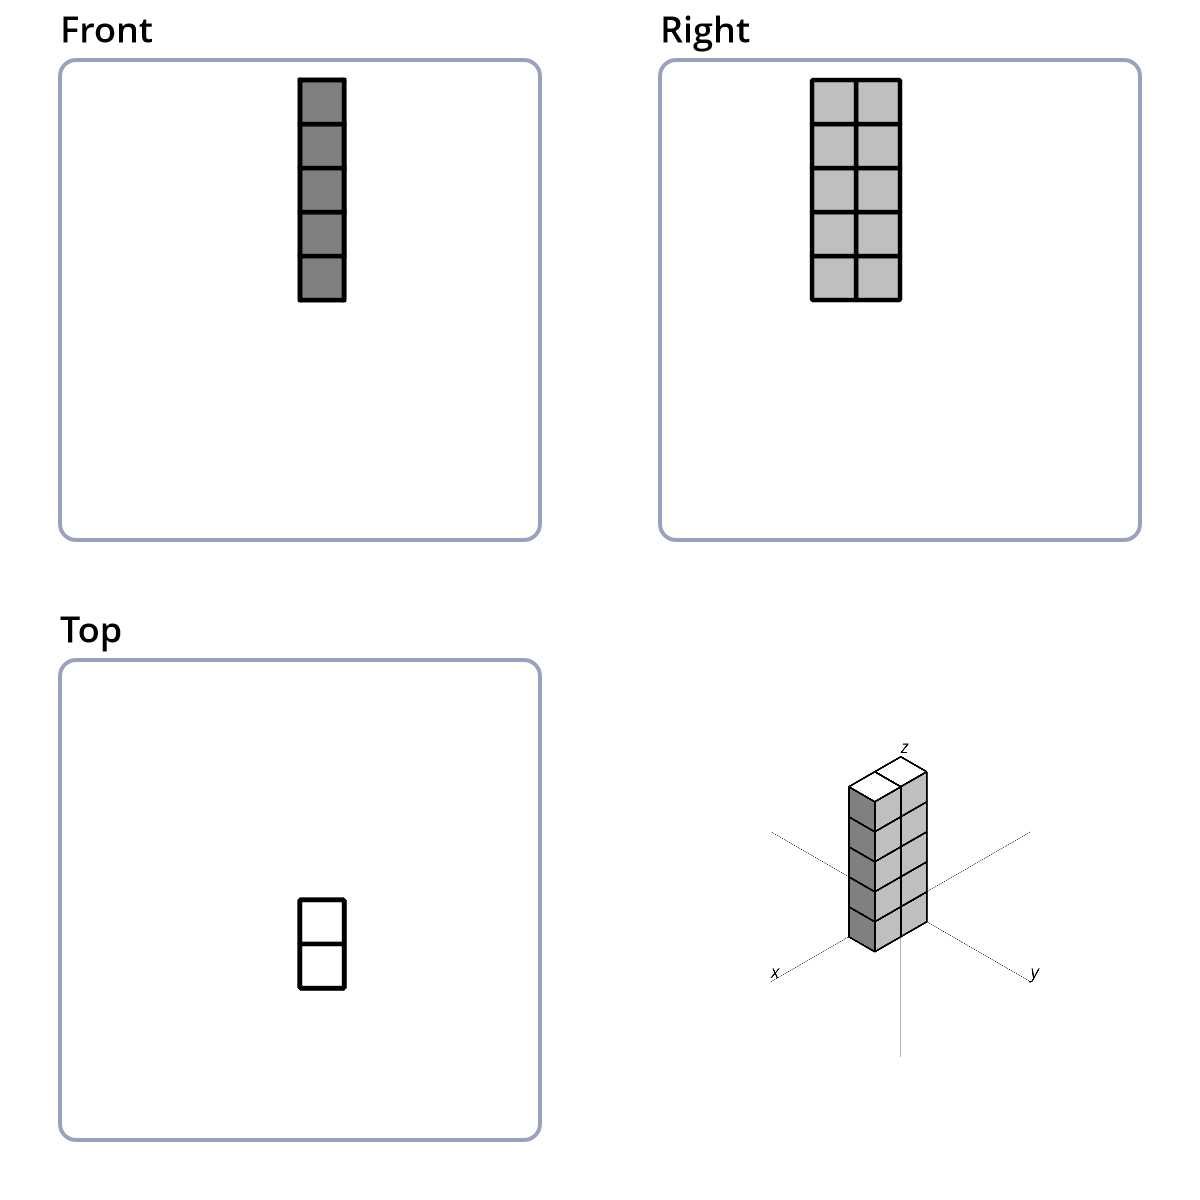
\includegraphics[scale=0.3]{iso_diagrams/o.png}
	\caption{Isometric of the O-pentomino.}
  \label{fig:iso-pent-o}
\end{figure}

\begin{figure}
	\centering
	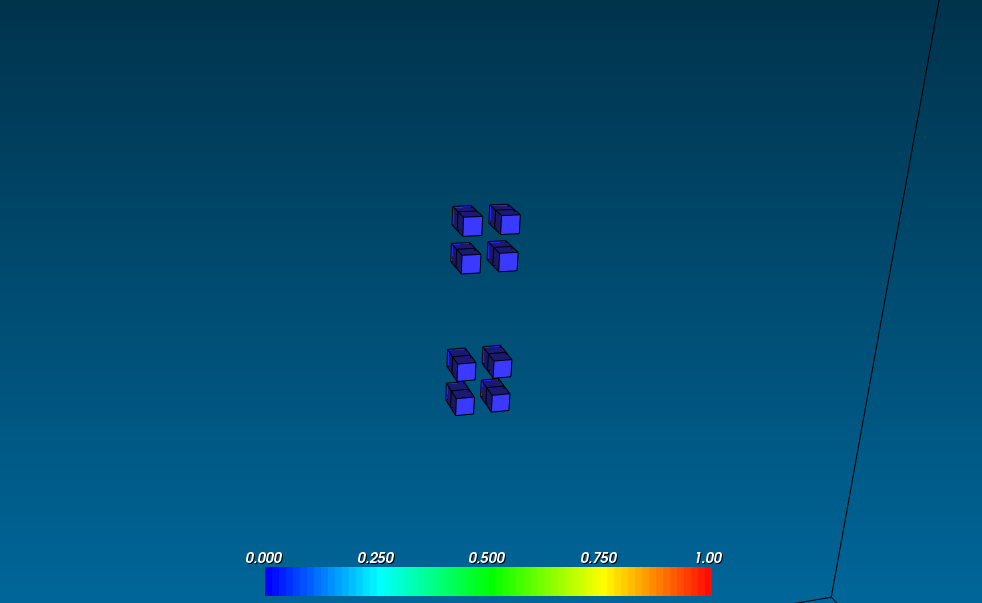
\includegraphics[scale=0.3]{pentominoes_ss/o_osc.png}
	\caption{Evolution of the O-Pentomino, $9^{th}$ generation.}
  \label{fig:ss-pent:o-osc}
\end{figure}

% P PENTOMINO ==================================================================
\subsubsection{P-Pentomino}
\label{sec:p-pentomino}

This pentomino (see figure~\ref{fig:iso-pent-p}) is quite interesting; three
configurations can be seen within less than 47 generations. The first one to
appear is a replicator (see figure~\ref{fig:iso-puffer-1}), latter, the first
(and one of the simplest) glider appears (see figure~\ref{fig:iso-glider-1});
finally, another glider appears (see figure~\ref{fig:iso-glider-2}).

Figure~\ref{fig:ss-pent:p-42} shows the state of the evolution of the
p-pentomino in the $42^{th}$ generation; the replicator can be seen in the north
of the evolution; while the gliders are located in the south of the population;
in~\ref{fig:ss-pent:p-42-puffer} the replicator can be seen in the left of the
figure and in~\ref{fig:ss-pent:p-42-glider}, the gliders can be seen in the
south.

The simulation of this pentomino stopped at 210 generations because space
was overcrowded.

\begin{figure}
	\centering
	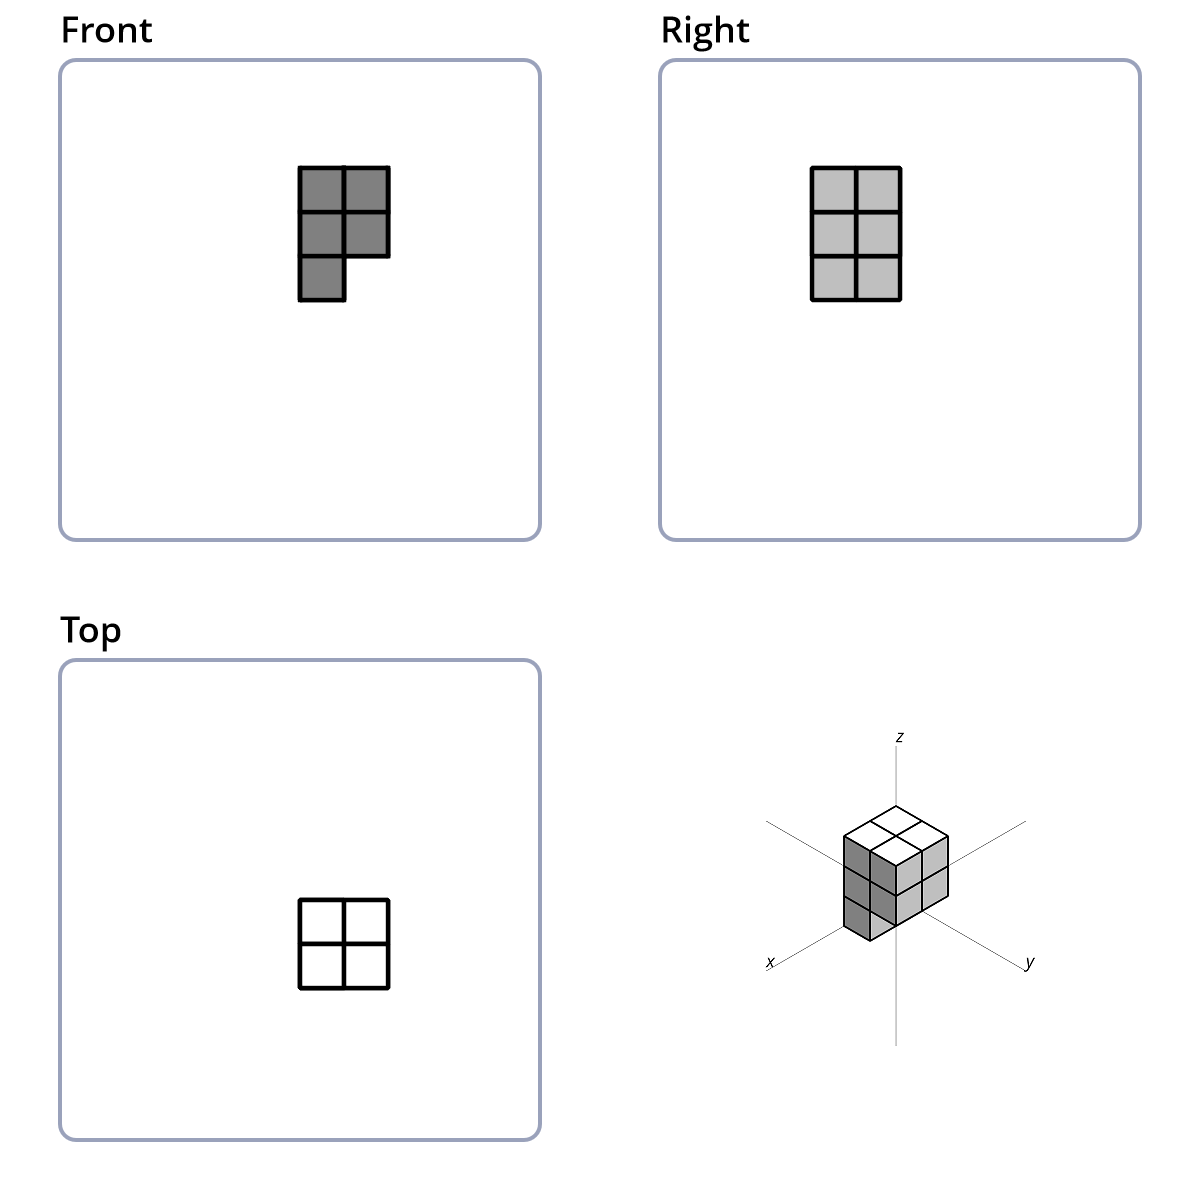
\includegraphics[scale=0.3]{iso_diagrams/p.png}
	\caption{Isometric of the P-pentomino.}
  \label{fig:iso-pent-p}
\end{figure}


\begin{figure}
	\centering
	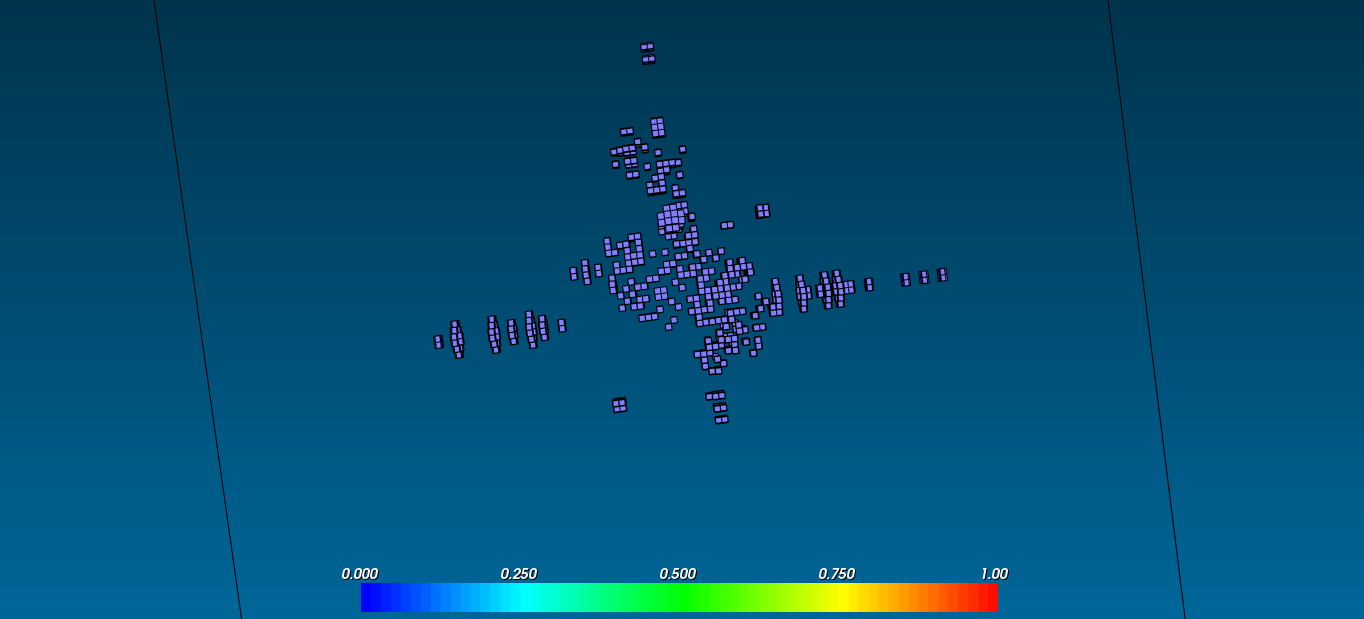
\includegraphics[scale=0.3]{pentominoes_ss/p_42.png}
	\caption{Evolution of the P-Pentomino, $42^{nd}$ generation.}
  \label{fig:ss-pent:p-42}
\end{figure}

\begin{figure}
	\centering
	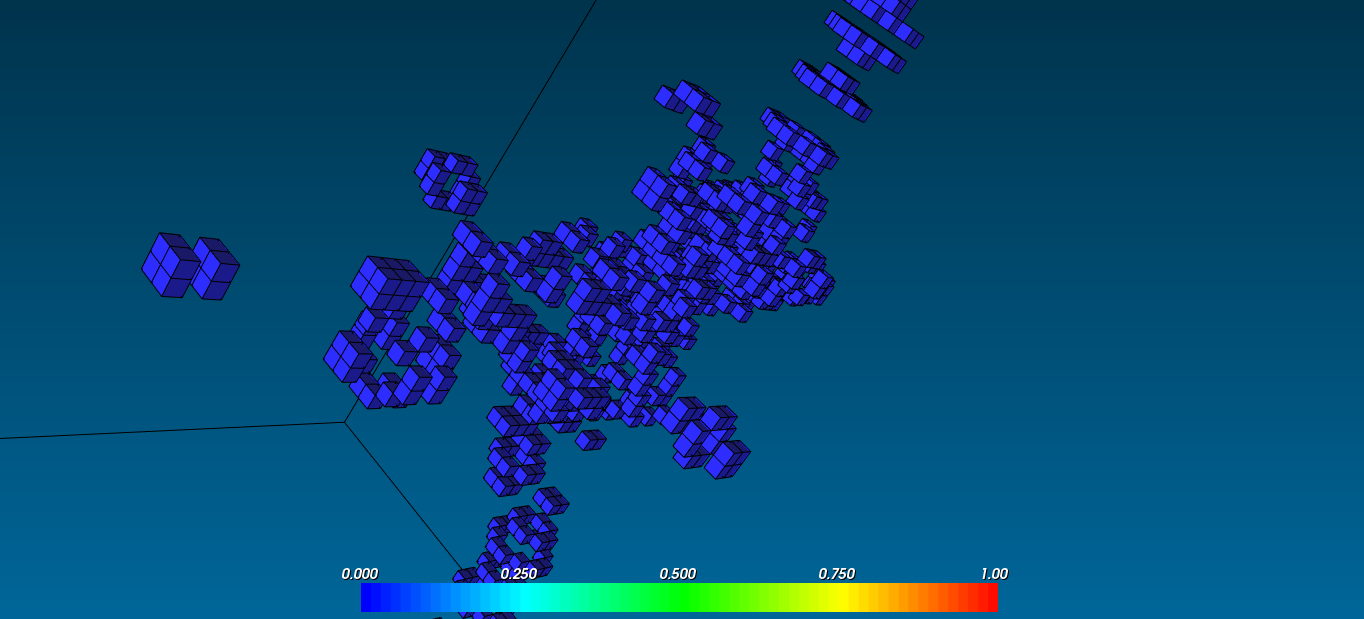
\includegraphics[scale=0.3]{pentominoes_ss/p_42_puffer.png}
	\caption{Evolution of the P-Pentomino, zoomed replicator, $42^{nd}$
	generation.}
  \label{fig:ss-pent:p-42-puffer}
\end{figure}

\begin{figure}
	\centering
	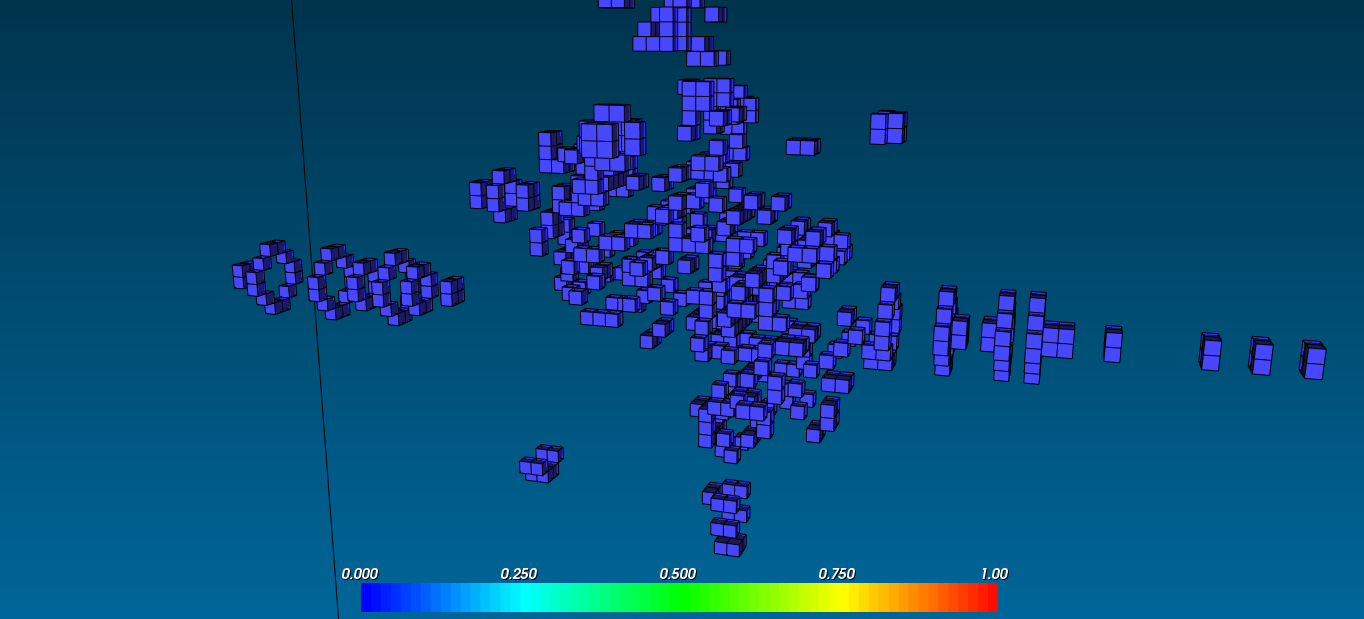
\includegraphics[scale=0.3]{pentominoes_ss/p_42_gliders.png}
	\caption{Evolution of the P-Pentomino, zoomed gliders, $42^{nd}$ generation.}
  \label{fig:ss-pent:p-42-glider}
\end{figure}


% Q PENTOMINO ==================================================================
\subsubsection{Q-Pentomino}
\label{sec:q-pentomino}
This pentomino (see figure~\ref{fig:iso-pent-q}) shows in ten generations, two
structures, one is the replicator-1 (see figure~\ref{fig:iso-puffer-1}), and a
\textit{modified} glider: the glider-1 (see figure~\ref{fig:iso-glider-1}) with
a satellite (see figure~\ref{fig:iso-glider-3}). The evolution of the $10^{th}$
generation with both structures can be seen in figure~\ref{fig:ss-pent:q-10}.

As shown in~\ref{fig:ss-pent:q-50}, in the $50^{th}$ generation, a mirrored
glider-4 (see figure~\ref{fig:iso-glider-4}) emerges, both in the north and
south of the population; the figures \ref{fig:ss-pent:q-50-gliders} and
\ref{fig:ss-pent:q-52-gliders} show the gliders, zoomed, in the $50^{th}$ and
$52^{nd}$ generation, respectively.

The simulation of this pentomino stopped at 109 generations because space
was overcrowded.

\begin{figure}
	\centering
	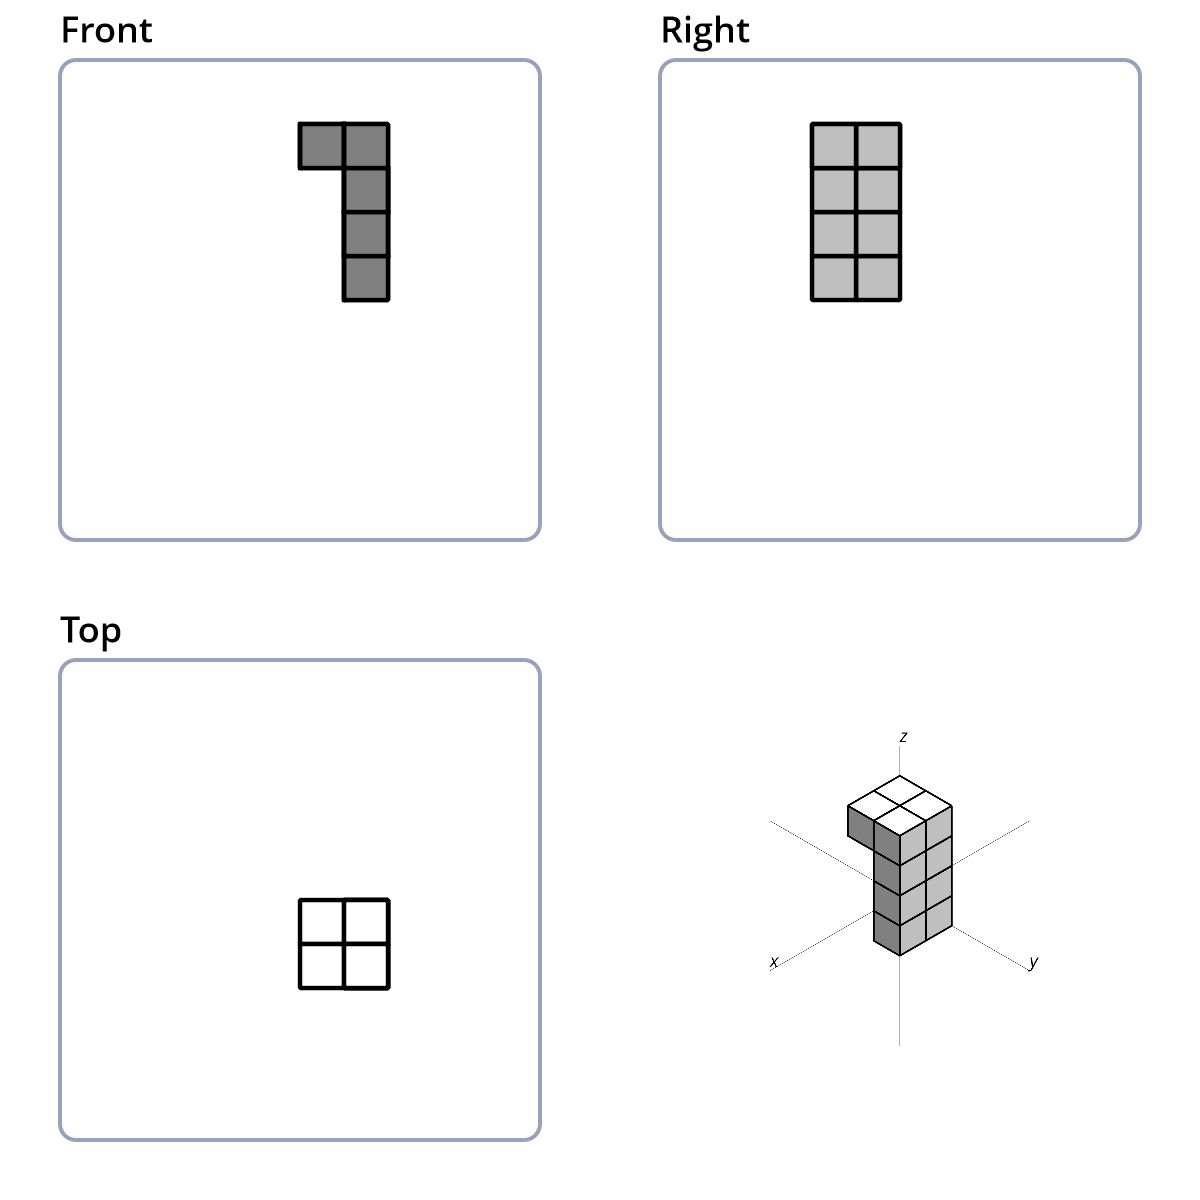
\includegraphics[scale=0.3]{iso_diagrams/q.png}
	\caption{Isometric of the Q-pentomino.}
  \label{fig:iso-pent-q}
\end{figure}

\begin{figure}
	\centering
	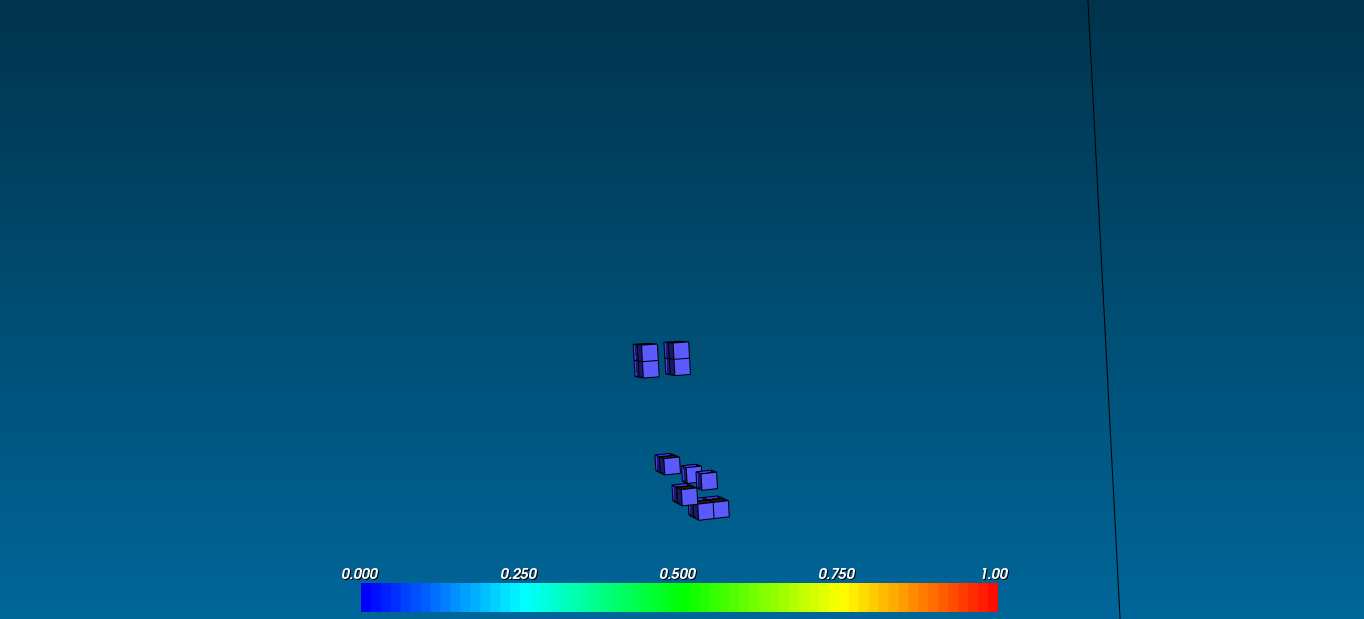
\includegraphics[scale=0.3]{pentominoes_ss/q_10.png}
	\caption{Evolution of the Q-Pentomino, $10^{th}$ generation.}
  \label{fig:ss-pent:q-10}
\end{figure}

\begin{figure}
	\centering
	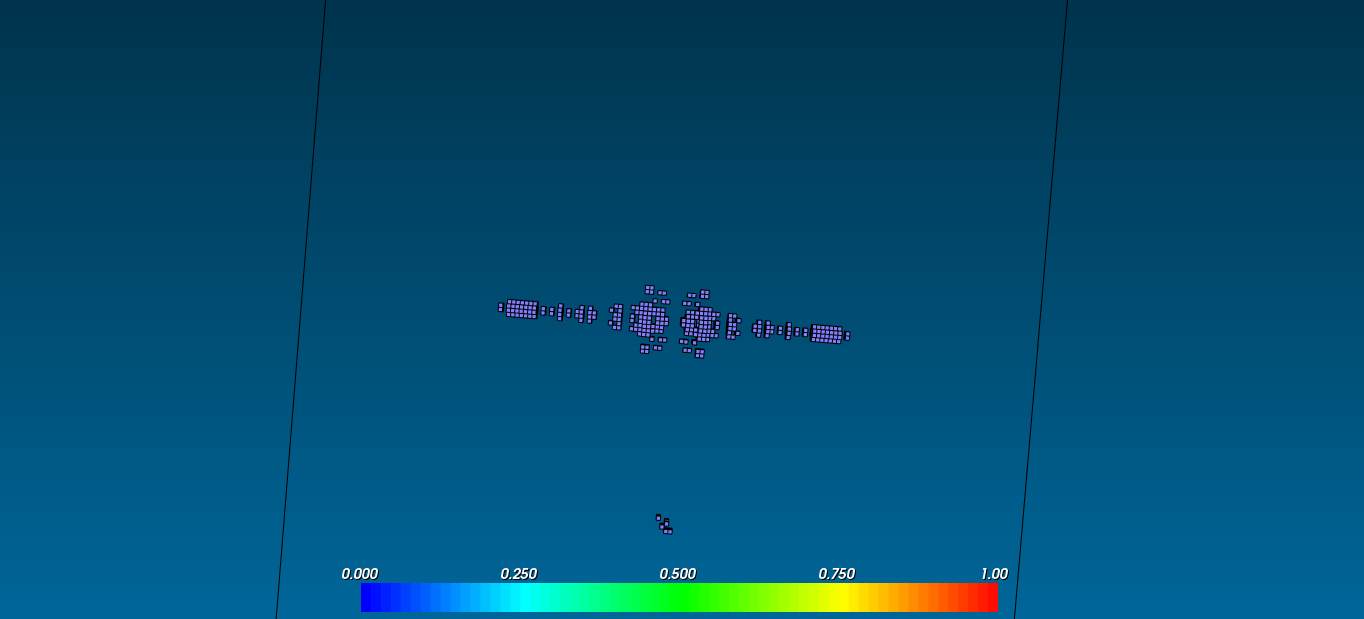
\includegraphics[scale=0.3]{pentominoes_ss/q_50.png}
	\caption{Evolution of the Q-Pentomino, $50^{th}$ generation.}
  \label{fig:ss-pent:q-50}
\end{figure}

\begin{figure}
	\centering
	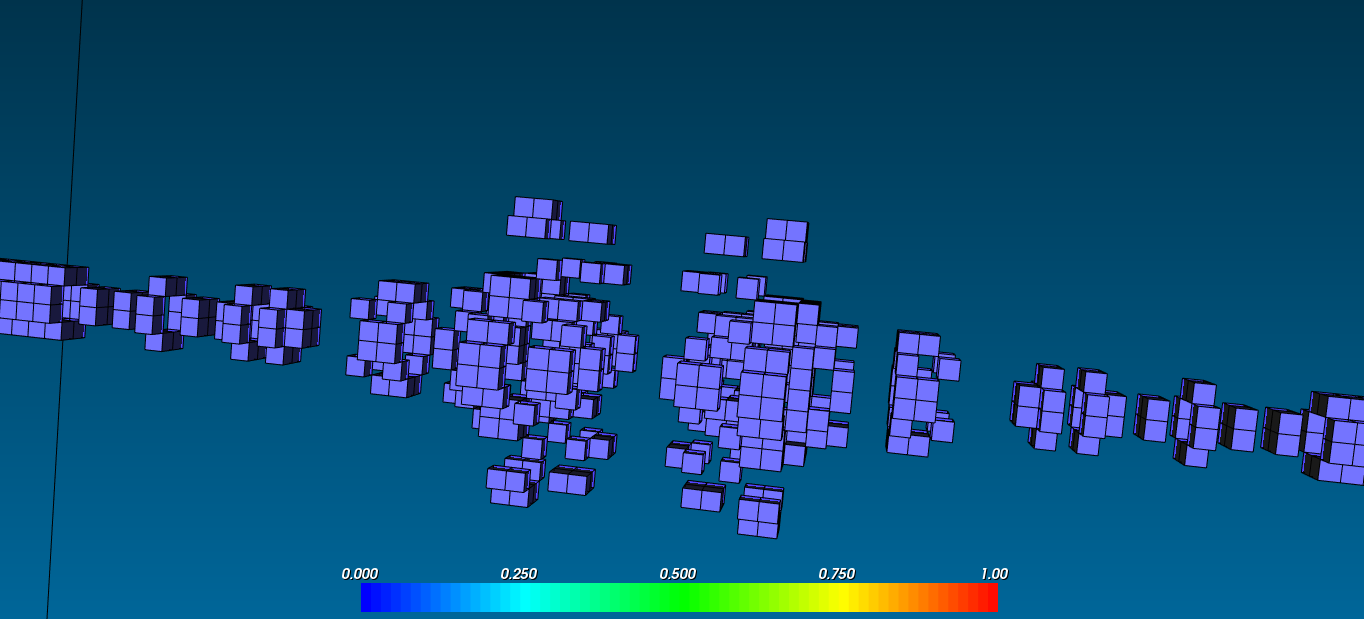
\includegraphics[scale=0.3]{pentominoes_ss/q_50_gliders.png}
	\caption{Evolution of the Q-Pentomino, zoomed gliders, $50^{th}$ generation.}
  \label{fig:ss-pent:q-50-gliders}
\end{figure}

\begin{figure}
	\centering
	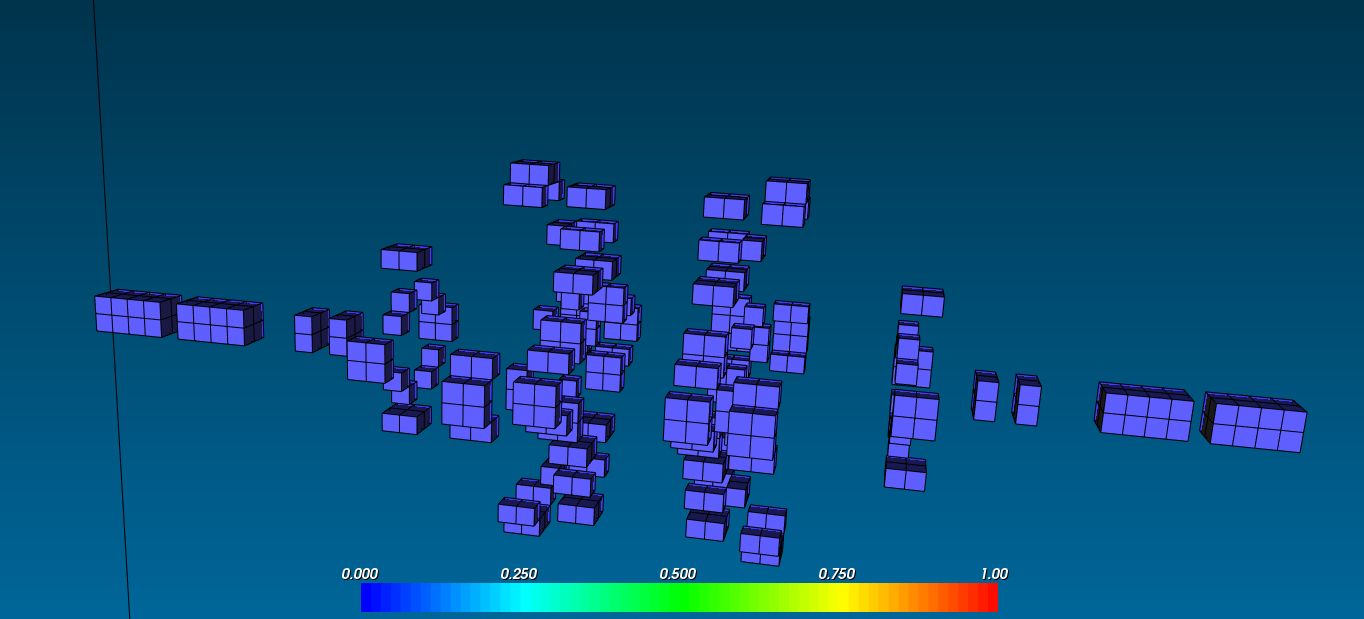
\includegraphics[scale=0.3]{pentominoes_ss/q_52_gliders.png}
	\caption{Evolution of the Q-Pentomino, zoomed gliders, $52^{nd}$ generation.}
  \label{fig:ss-pent:q-52-gliders}
\end{figure}

% R PENTOMINO ==================================================================
\subsubsection{R-Pentomino}
\label{sec:r-pentomino}
This pentomino (see figure~\ref{fig:iso-pent-r}), just like it's equivalent in
two dimensions, expands very quickly in a short period of time, this can be
observed in figure~\ref{fig:ss-pent:r-comparative}, where a comparison between
the evolution achieved in the same generation for different pentominoes.

The replicator (see figure~\ref{fig:iso-puffer-1}) appears here, too; as the
glider-1 (see figure~\ref{fig:iso-glider-1}) and glider-4 (see
figure~\ref{fig:iso-glider-4}); the gliders can be seen in the  $81^{st}$
generation, in the north-east, north-west, south-east and south-west areas of
figure~\ref{fig:ss-pent:r-81}; in figure~\ref{fig:ss-pent:r-81-glider1}, a
pair of glider-1 can be seen easily in the left of the figure; the glider-4 is
shown in the upper-left of figure~\ref{fig:ss-pent:r-81-glider4}.

\begin{figure}
	\centering
	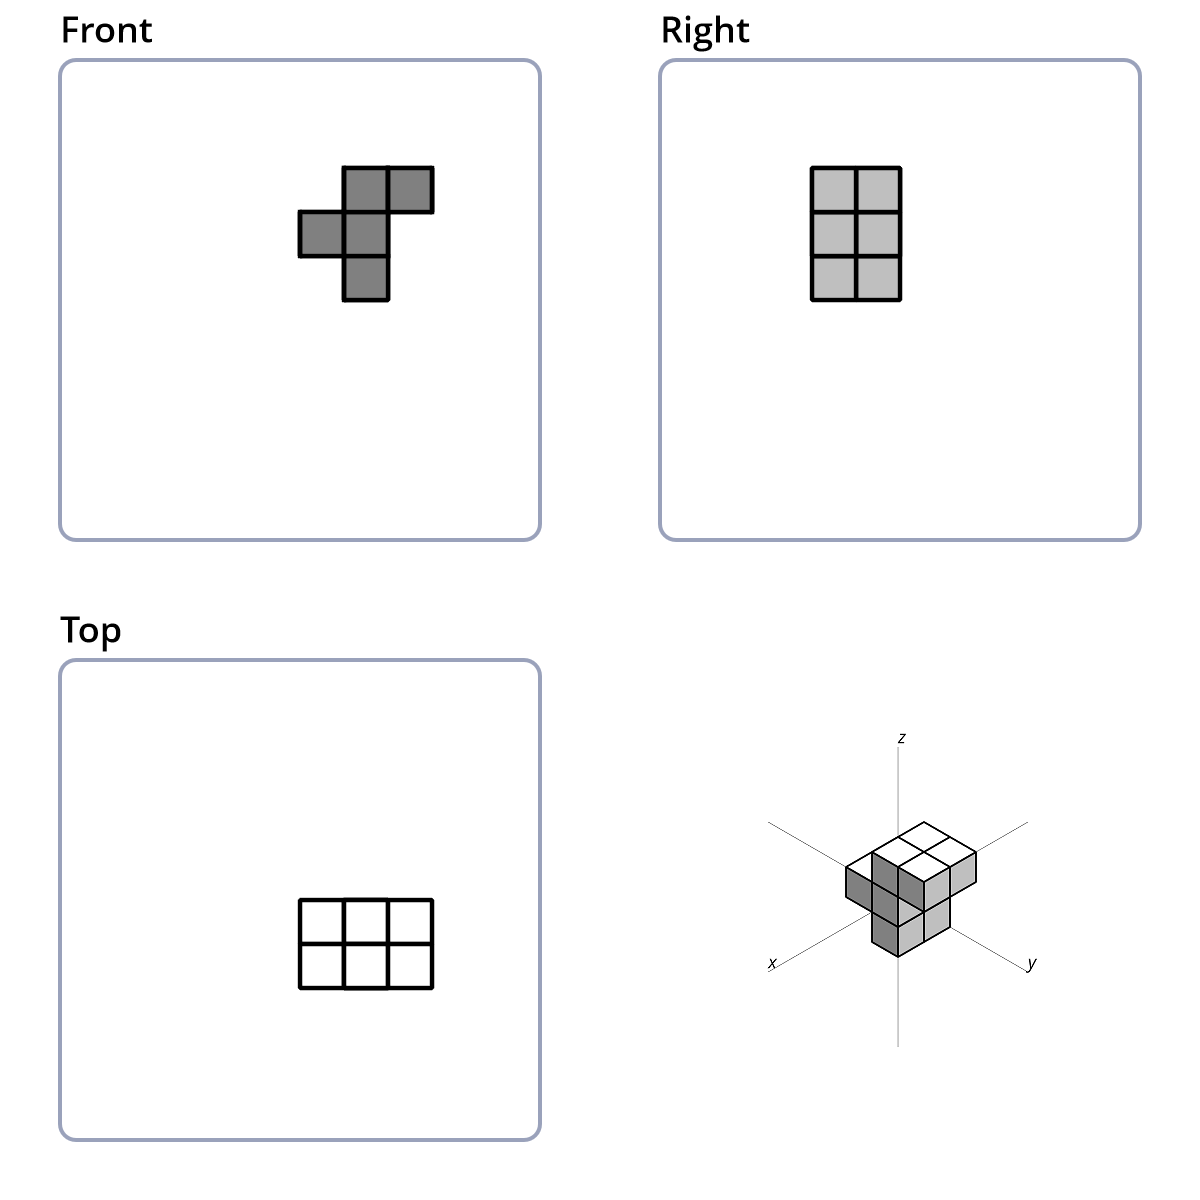
\includegraphics[scale=0.3]{iso_diagrams/r.png}
	\caption{Isometric of the R-pentomino.}
  \label{fig:iso-pent-r}
\end{figure}

\begin{figure}
	\centering
	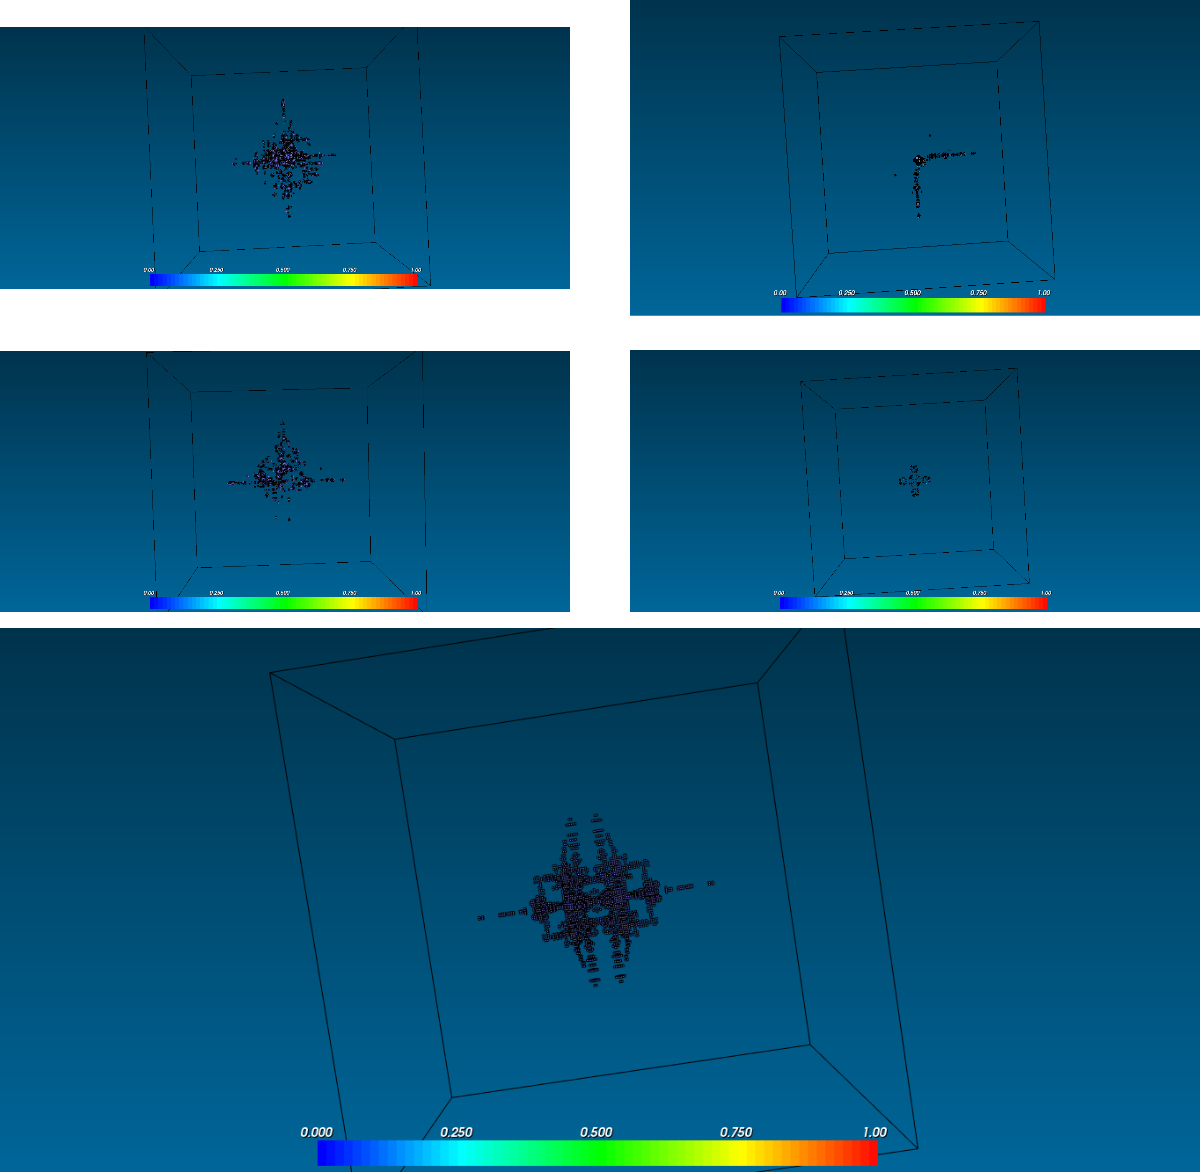
\includegraphics[scale=0.4]{pentominoes_ss/r-comparative-70g.png}
	\caption{Evolution in the $52^{th}$ generation for the Y, W, P, X and R
	pentominoes respectively.}
  \label{fig:ss-pent:r-comparative}
\end{figure}

\begin{figure}
	\centering
	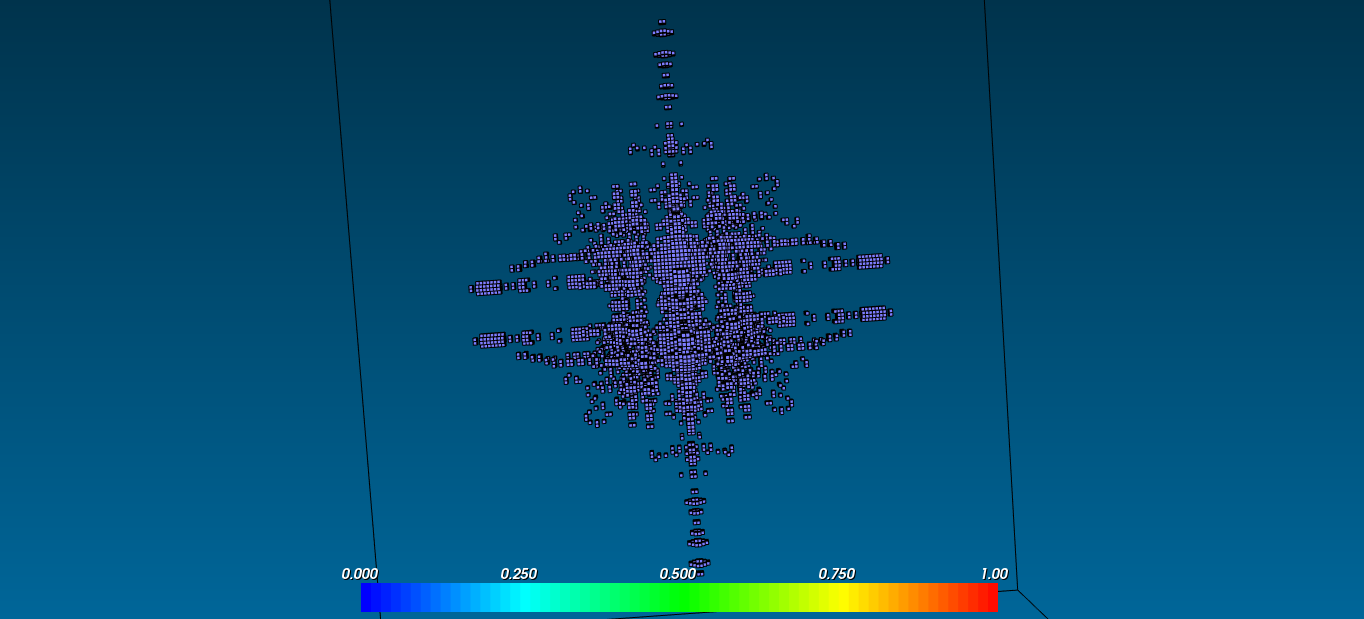
\includegraphics[scale=0.3]{pentominoes_ss/r_81.png}
	\caption{Evolution of the R-Pentomino, $81^{st}$ generation.}
  \label{fig:ss-pent:r-81}
\end{figure}

\begin{figure}
	\centering
	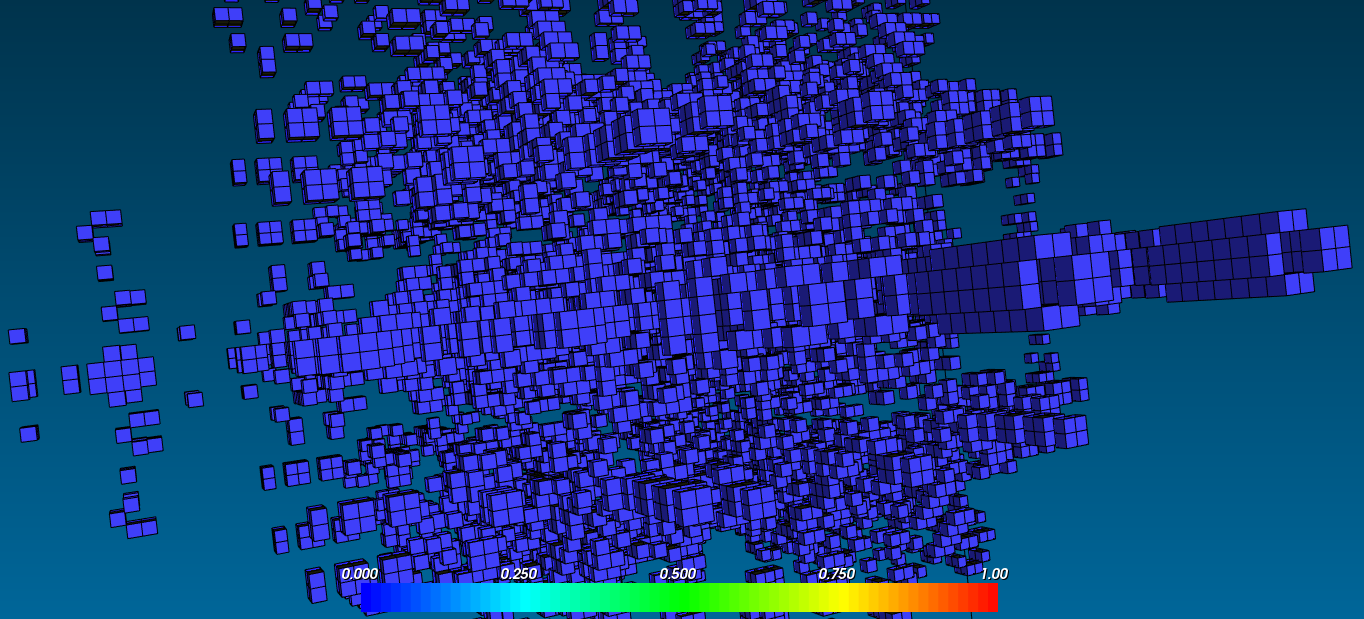
\includegraphics[scale=0.3]{pentominoes_ss/r_81_glider1.png}
	\caption{Evolution of the R-Pentomino, zoomed glider-1, $81^{st}$ generation.}
  \label{fig:ss-pent:r-81-glider1}
\end{figure}

\begin{figure}
	\centering
	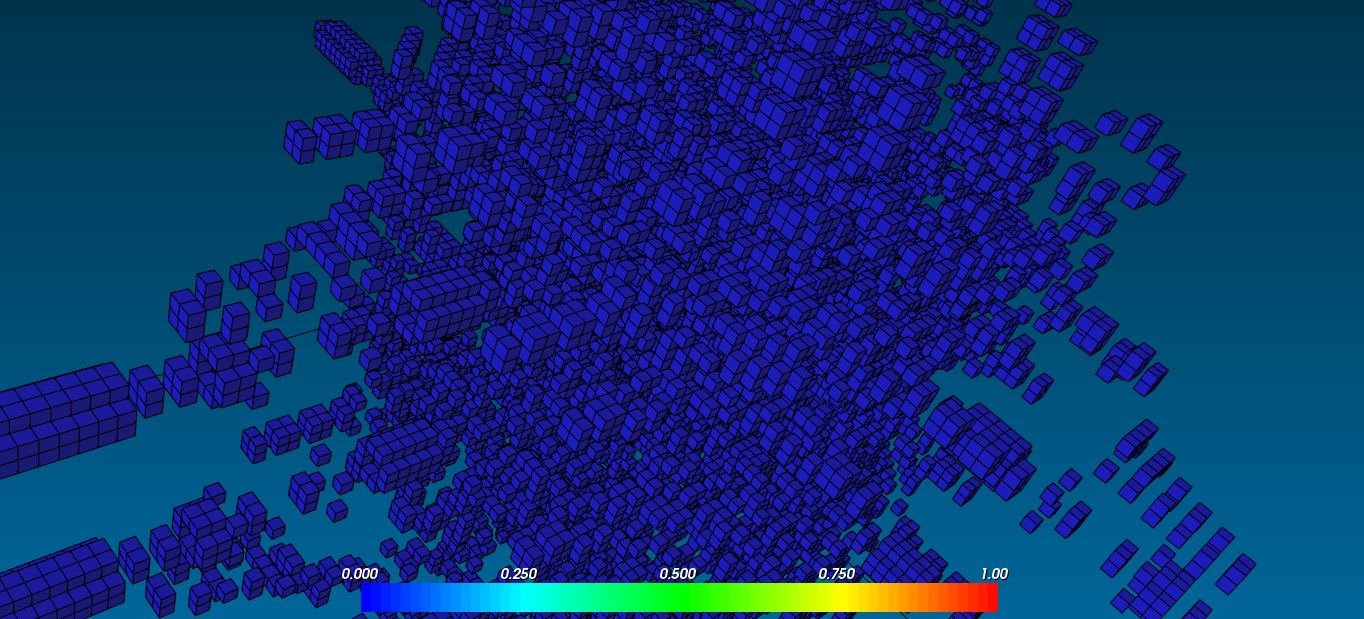
\includegraphics[scale=0.3]{pentominoes_ss/r_81_glider4.png}
	\caption{Evolution of the R-Pentomino, zoomed glider-4, $81^{st}$ generation.}
  \label{fig:ss-pent:r-81-glider4}
\end{figure}

% S PENTOMINO ==================================================================
\subsubsection{S-Pentomino}
\label{sec:s-pentomino}
This pentomino (see figure~\ref{fig:iso-pent-s}) shows, quite fast, the
replicator-1, seen in previous pentominoes first; later a clean puffer
(see figure~\ref{fig:iso-puffer-2}) emerges; four of these puffers can be
observed in figure~\ref{fig:ss-pent:s-56}. This was one of the most active
pentominoes; and, although the simulation had to be stopped after 131
generations. Interestingly, the growth in the population seemed more ordered,
symmetrical and configuration driven: seems easier to find individual
configurations in the s-pentomino than in the others. Two pairs of puffer-2
can be seen again, a pair moving towards the east, and the other towards west;
in figures \ref{fig:ss-pent:s-57}~and~\ref{fig:ss-pent:s-59}.

\begin{figure}
	\centering
	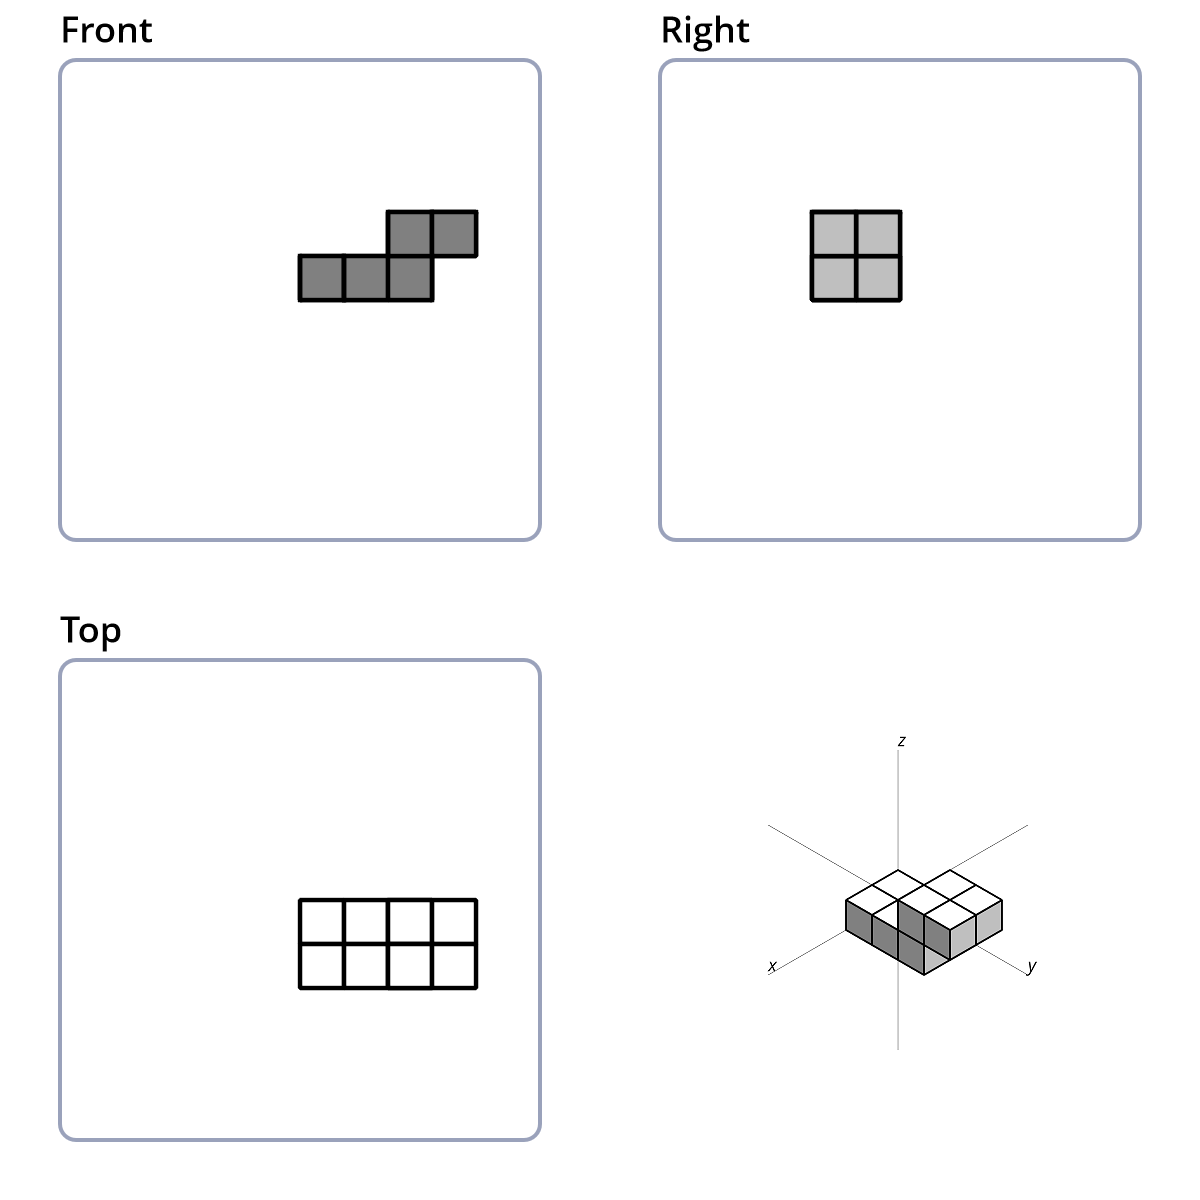
\includegraphics[scale=0.3]{iso_diagrams/s.png}
	\caption{Isometric of the S-pentomino.}
  \label{fig:iso-pent-s}
\end{figure}

\begin{figure}
	\centering
	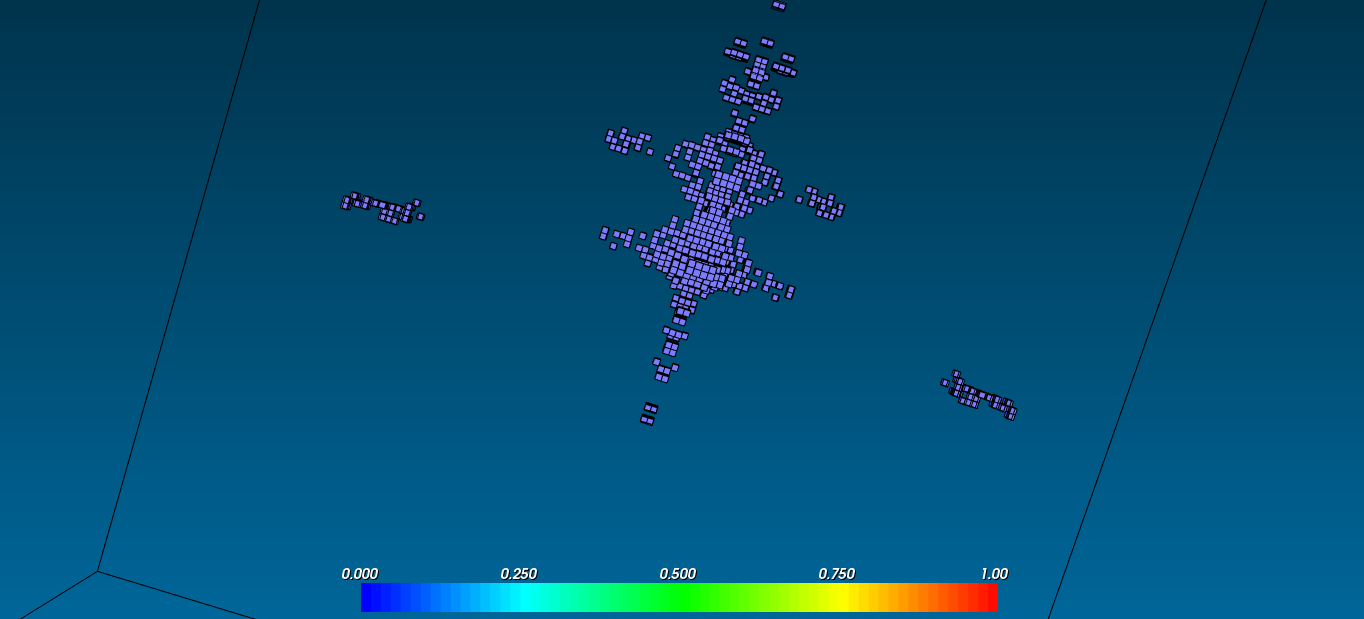
\includegraphics[scale=0.3]{pentominoes_ss/s_56.png}
	\caption{Evolution of the S-Pentomino, $56^{th}$ generation.}
  \label{fig:ss-pent:s-56}
\end{figure}

\begin{figure}
	\centering
	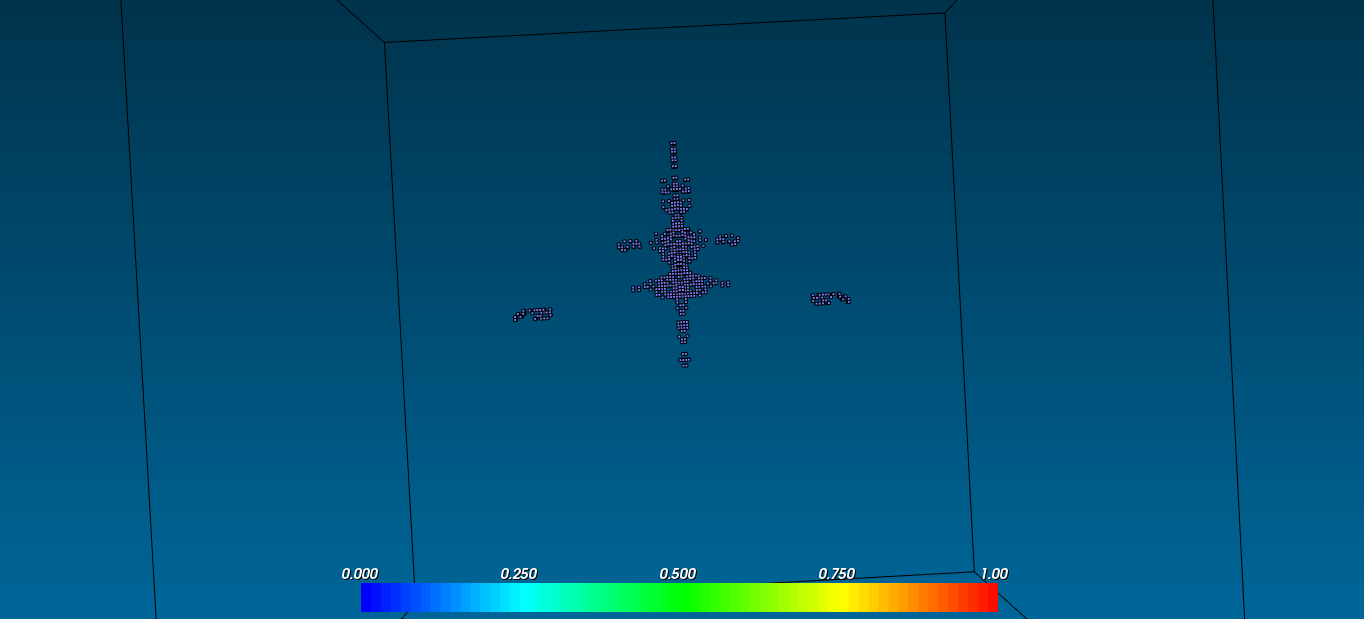
\includegraphics[scale=0.3]{pentominoes_ss/s_57.png}
	\caption{Evolution of the S-Pentomino, $57^{th}$ generation.}
  \label{fig:ss-pent:s-57}
\end{figure}

\begin{figure}
	\centering
	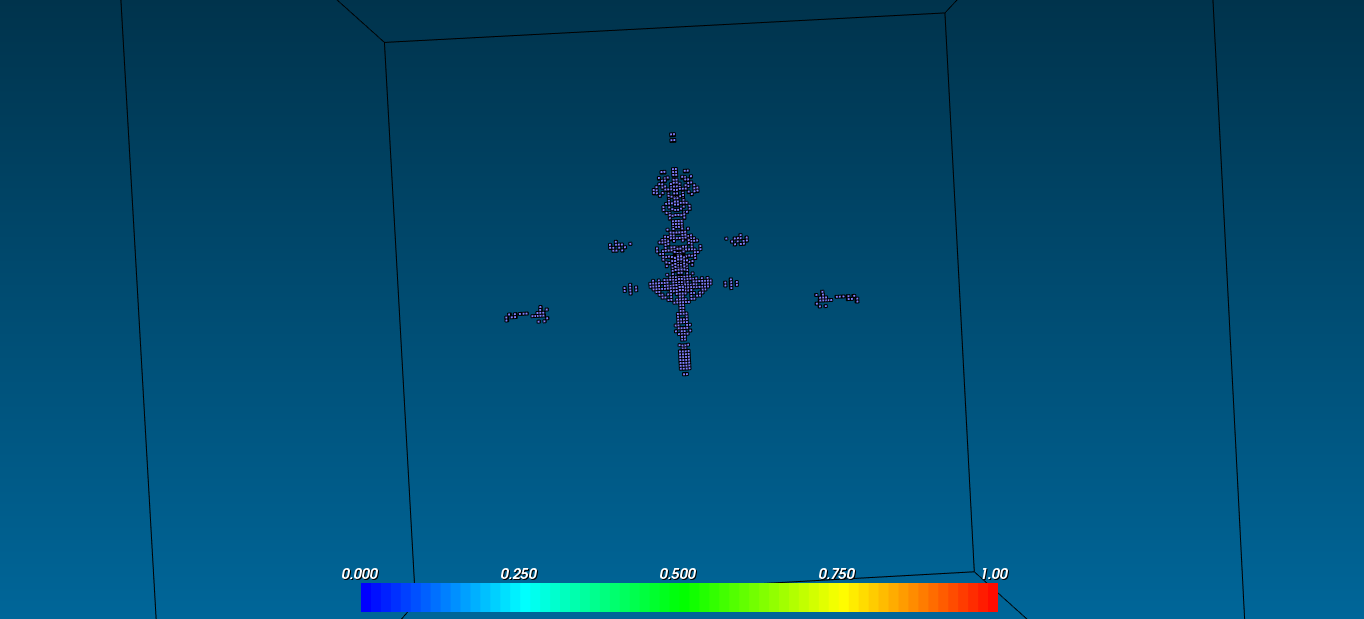
\includegraphics[scale=0.3]{pentominoes_ss/s_60.png}
	\caption{Evolution of the S-Pentomino, $60^{th}$ generation.}
  \label{fig:ss-pent:s-59}
\end{figure}

% T PENTOMINO ==================================================================
\subsubsection{T-Pentomino}
\label{sec:t-pentomino}
This pentomino (see figure~\ref{fig:iso-pent-t}) behaves rather differently
than it's equivalents in other rules (and dimensions); instead of evolving in a
replicator, spaceship, pulsar or such, dies within five generations.

\begin{figure}
	\centering
	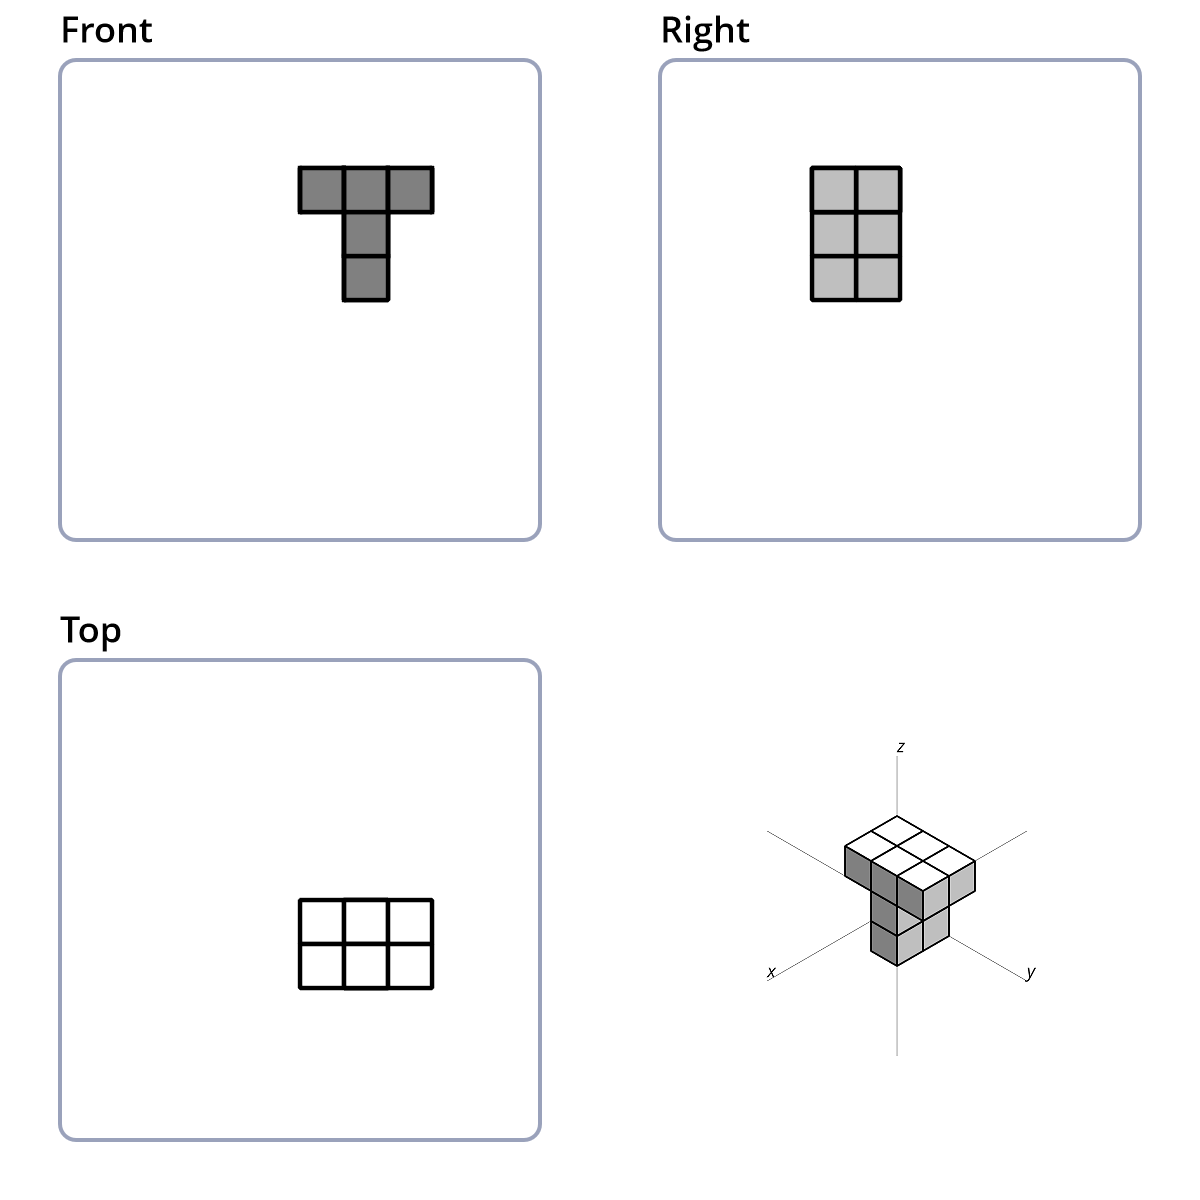
\includegraphics[scale=0.3]{iso_diagrams/t.png}
	\caption{Isometric of the T-pentomino.}
  \label{fig:iso-pent-t}
\end{figure}

% U PENTOMINO ==================================================================
\subsubsection{U-Pentomino}
\label{sec:u-pentomino}
This pentomino (see figure~\ref{fig:iso-pent-u}),shows the puffer-1 (see
figure~\ref{fig:iso-puffer-1v}) in less than 7 generations; unlike the puffer-2
(see figure~\ref{fig:iso-puffer-2}), this puffer is not clean at all and
pollutes very quickly. Interestingly enough, the population at its early stages
appears to be formed by configurations that look almost like gliders and puffers
found previously, but each fails a few cells. The glider-1 (see
figure~\ref{fig:iso-glider-1}) and the replicator-1 (see
figure~\ref{fig:iso-puffer-1}) appear heavily through the evolution of the
pentomino. A clean new puffer, the puffer-3 (see figure~\ref{fig:iso-puffer-3})
and a glider, the glider-5 (see figure~\ref{fig:iso-glider-5}, appear in this
pentomino; both, the new puffer and glider can be observed in
figure~\ref{fig:ss-pent:u-70}: the glider-5 in the north and the puffer-3 in the
north-east and east of the figure.

\begin{figure}
	\centering
	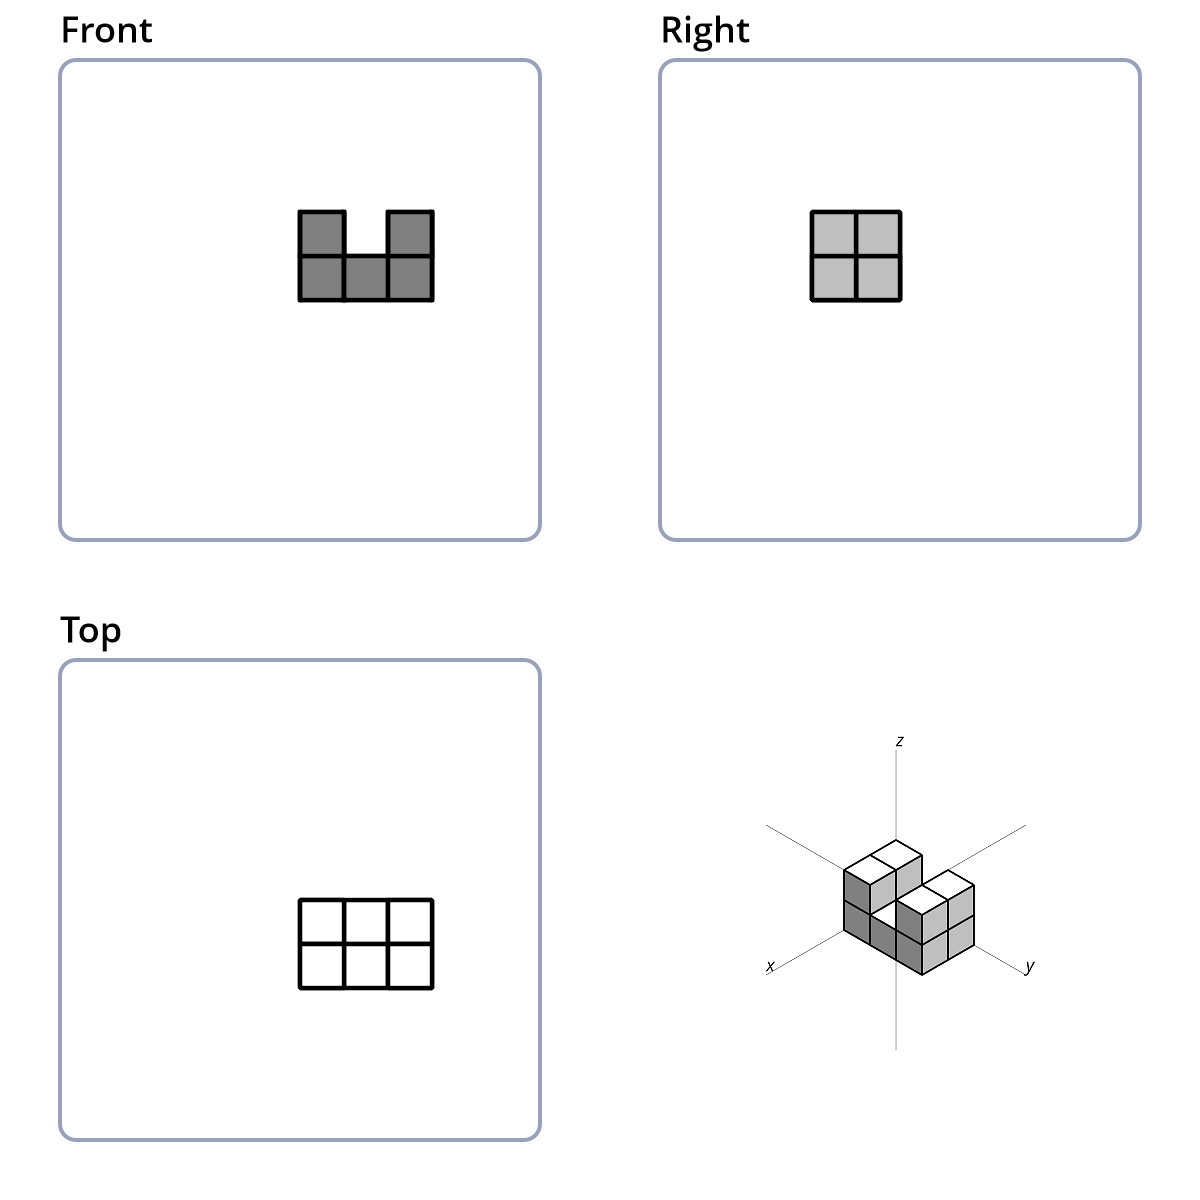
\includegraphics[scale=0.3]{iso_diagrams/u.png}
	\caption{Isometric of the U-pentomino.}
  \label{fig:iso-pent-u}
\end{figure}

\begin{figure}
	\centering
	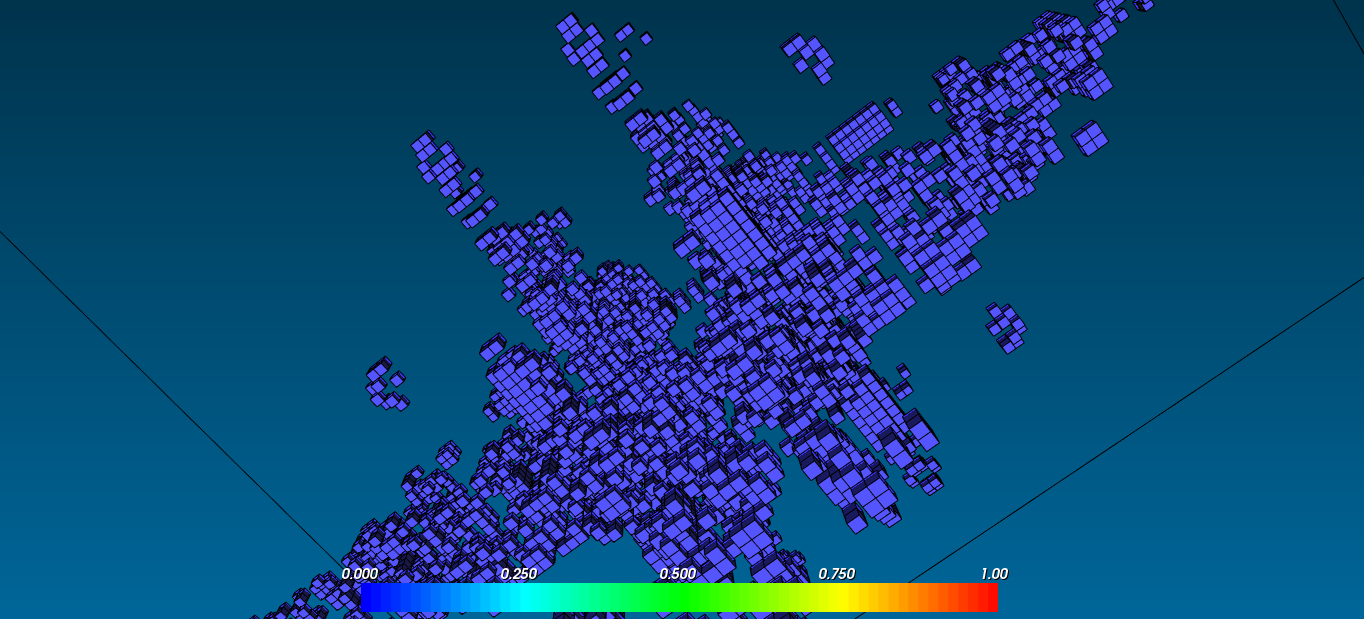
\includegraphics[scale=0.3]{pentominoes_ss/u_70.png}
	\caption{Evolution of the U-Pentomino, $70^{th}$ generation.}
	\label{fig:ss-pent:u-70}
\end{figure}

% V PENTOMINO ==================================================================
\subsubsection{V-Pentomino}
\label{sec:v-pentomino}

In this pentomino (see figure~\ref{fig:iso-pent-v}), a pair of replicator-1 (see
figure~\ref{fig:iso-puffer-1}) appear in the early stages of its evolution.
Although the replicator-1 starts by replicating itself in the z-axis, soon it
starts to replicate perpendicularly to itself, as observed in
figure~\ref{fig:ss-pent:v-48}.

\begin{figure}
	\centering
	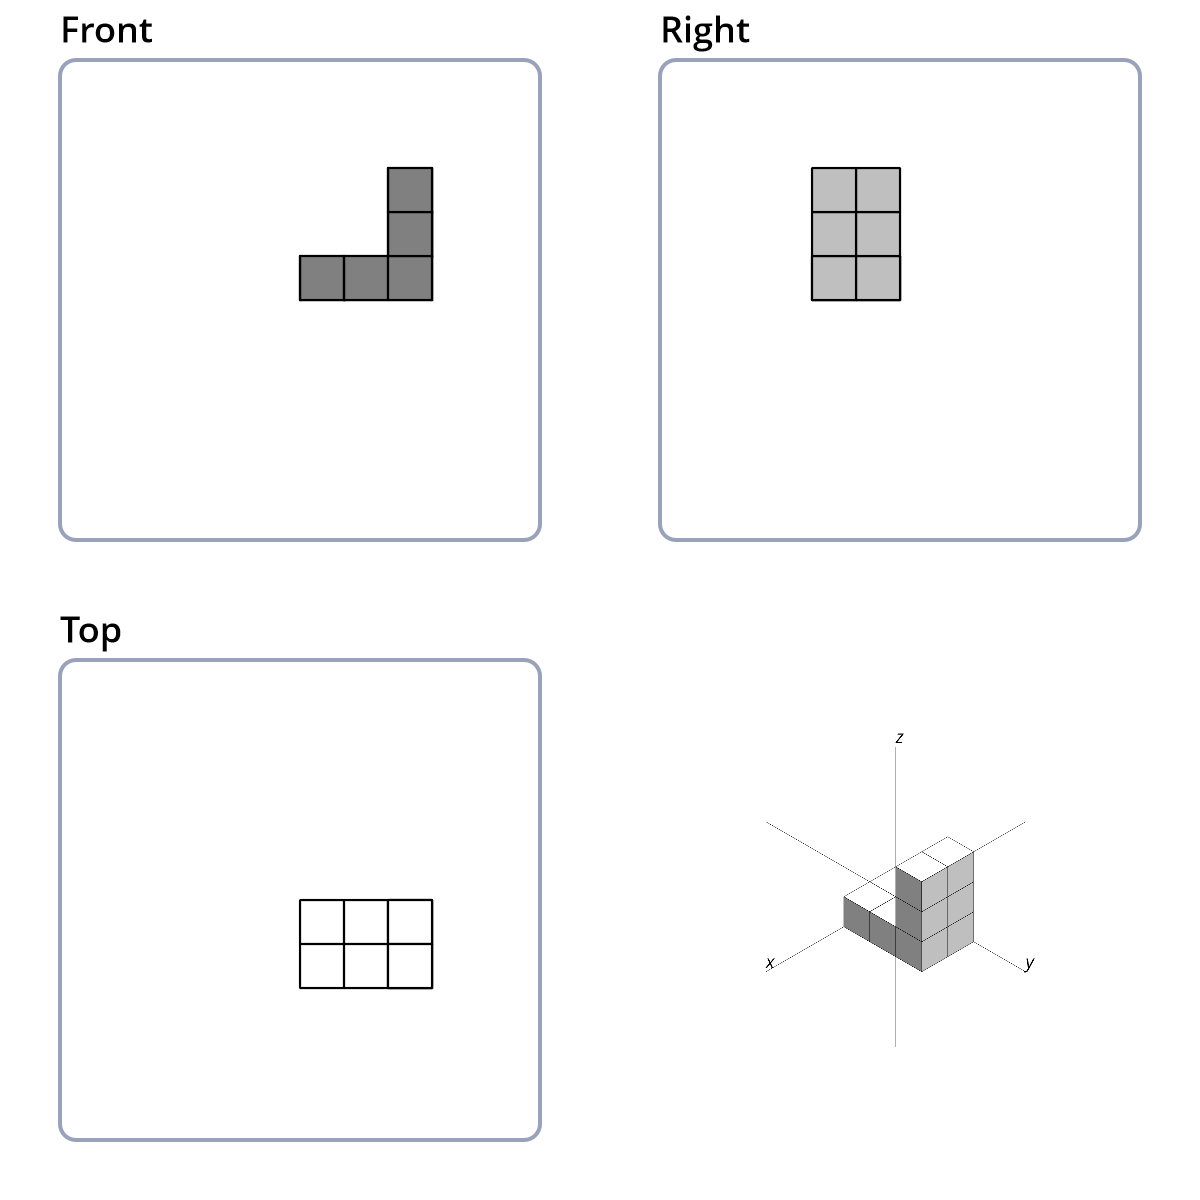
\includegraphics[scale=0.3]{iso_diagrams/v.png}
	\caption{Isometric of the V-pentomino.}
  \label{fig:iso-pent-v}
\end{figure}

\begin{figure}
	\centering
	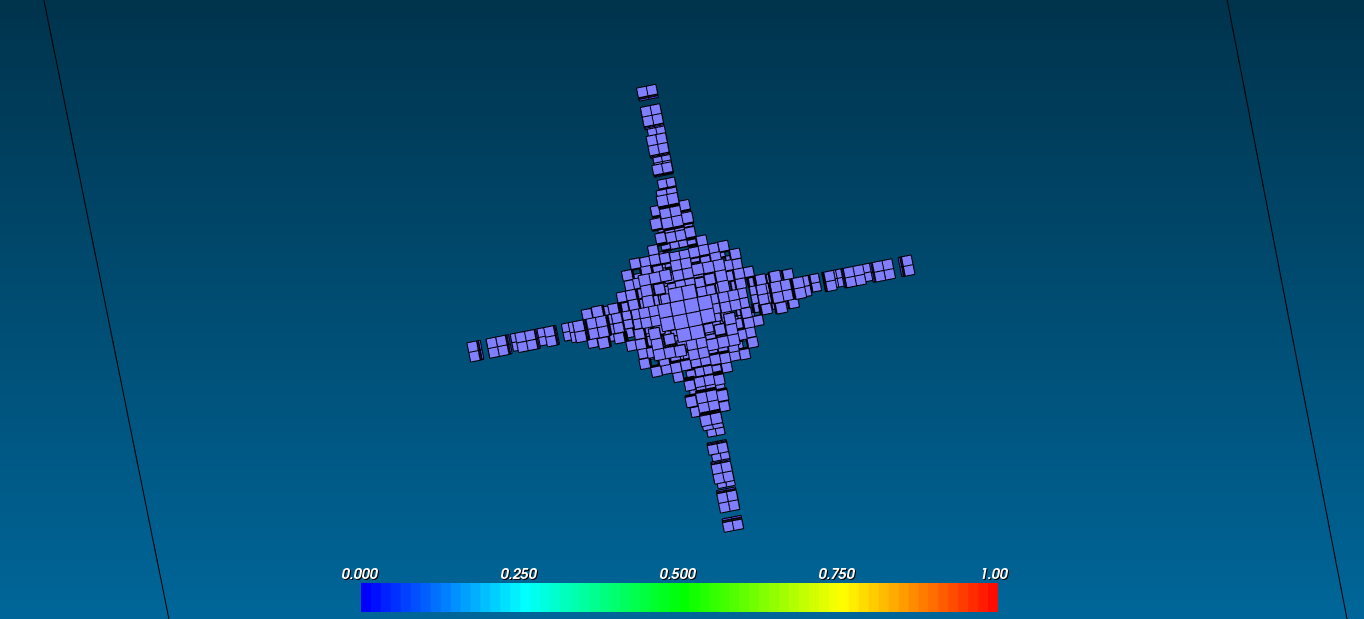
\includegraphics[scale=0.3]{pentominoes_ss/v_48.png}
	\caption{Evolution of the V-Pentomino, $48^{th}$ generation.}
	\label{fig:ss-pent:v-48}
\end{figure}

% W PENTOMINO ==================================================================
\subsubsection{W-Pentomino}
\label{sec:w-pentomino}
This pentomino (see figure~\ref{fig:iso-pent-w}), unlike its predecessor, the
V-pentomino, \textit{folds} since the beggining and the two initial replicator-1
start to replicate perpendicularly since the beginning  (see
figure~\ref{fig:ss-pent:w-12}).

\begin{figure}
	\centering
	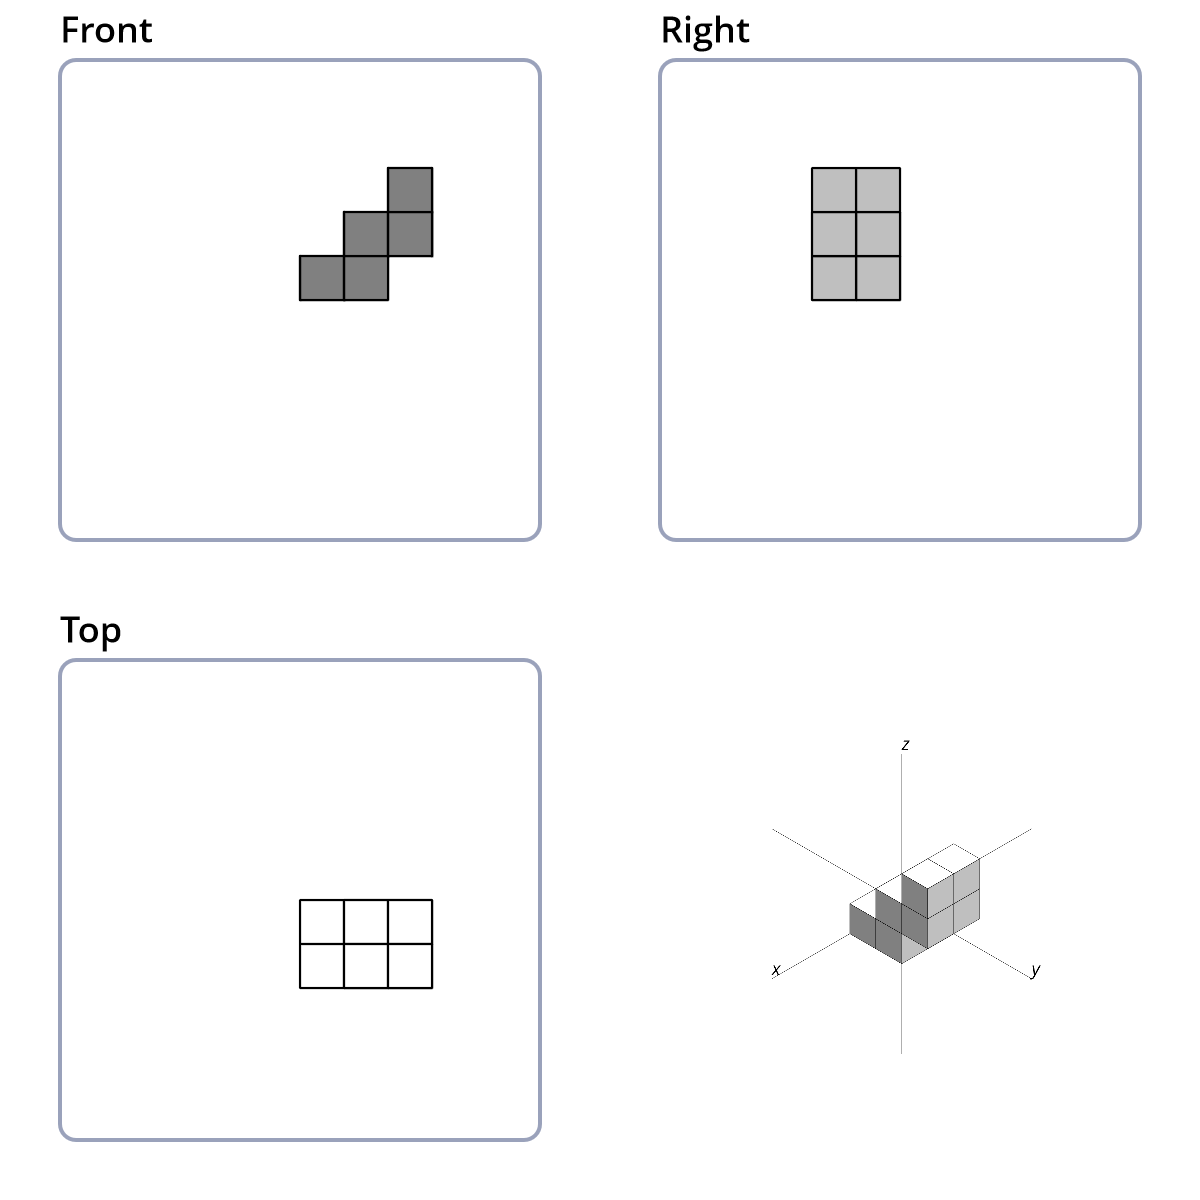
\includegraphics[scale=0.3]{iso_diagrams/w.png}
	\caption{Isometric of the W-pentomino.}
  \label{fig:iso-pent-w}
\end{figure}

\begin{figure}
	\centering
	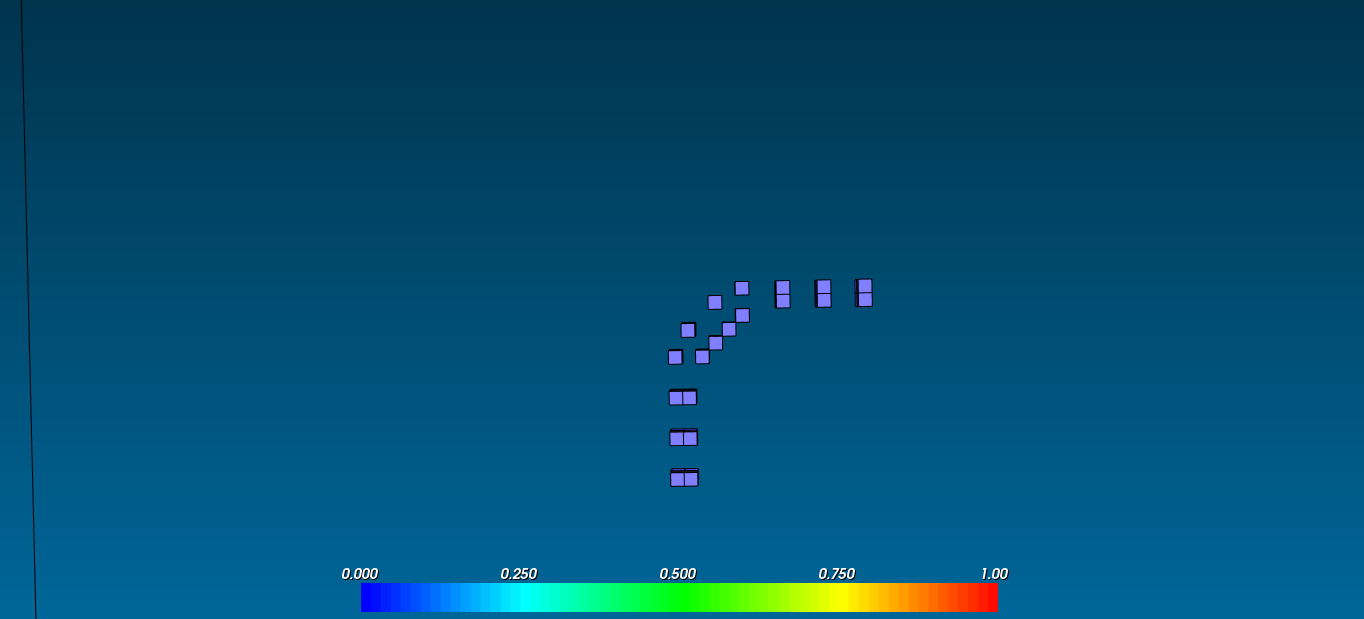
\includegraphics[scale=0.3]{pentominoes_ss/w_12.png}
	\caption{Evolution of the W-Pentomino, $12^{th}$ generation.}
	\label{fig:ss-pent:w-12}
\end{figure}

% X PENTOMINO ==================================================================
\subsubsection{X-Pentomino}
\label{sec:x-pentomino}
This pentomino's (see figure~\ref{fig:iso-pent-x}) first evolution's stages
appear to be related to the oscillator-1 (see figure~\ref{fig:iso-osc-1} for the
oscillator and figures \ref{fig:ss-pent:x-2}, \ref{fig:ss-pent:x-3},
\ref{fig:ss-pent:x-4}, \ref{fig:ss-pent:x-5}, \ref{fig:ss-pent:x-6} and
\ref{fig:ss-pent:x-7} for the pentomino's evolution). Then, as shown in
figure~\ref{fig:ss-pent:x-15}, it evolves into a set of replicator-1 (see
figure~\ref{fig:iso-puffer-1}).

\begin{figure}
	\centering
	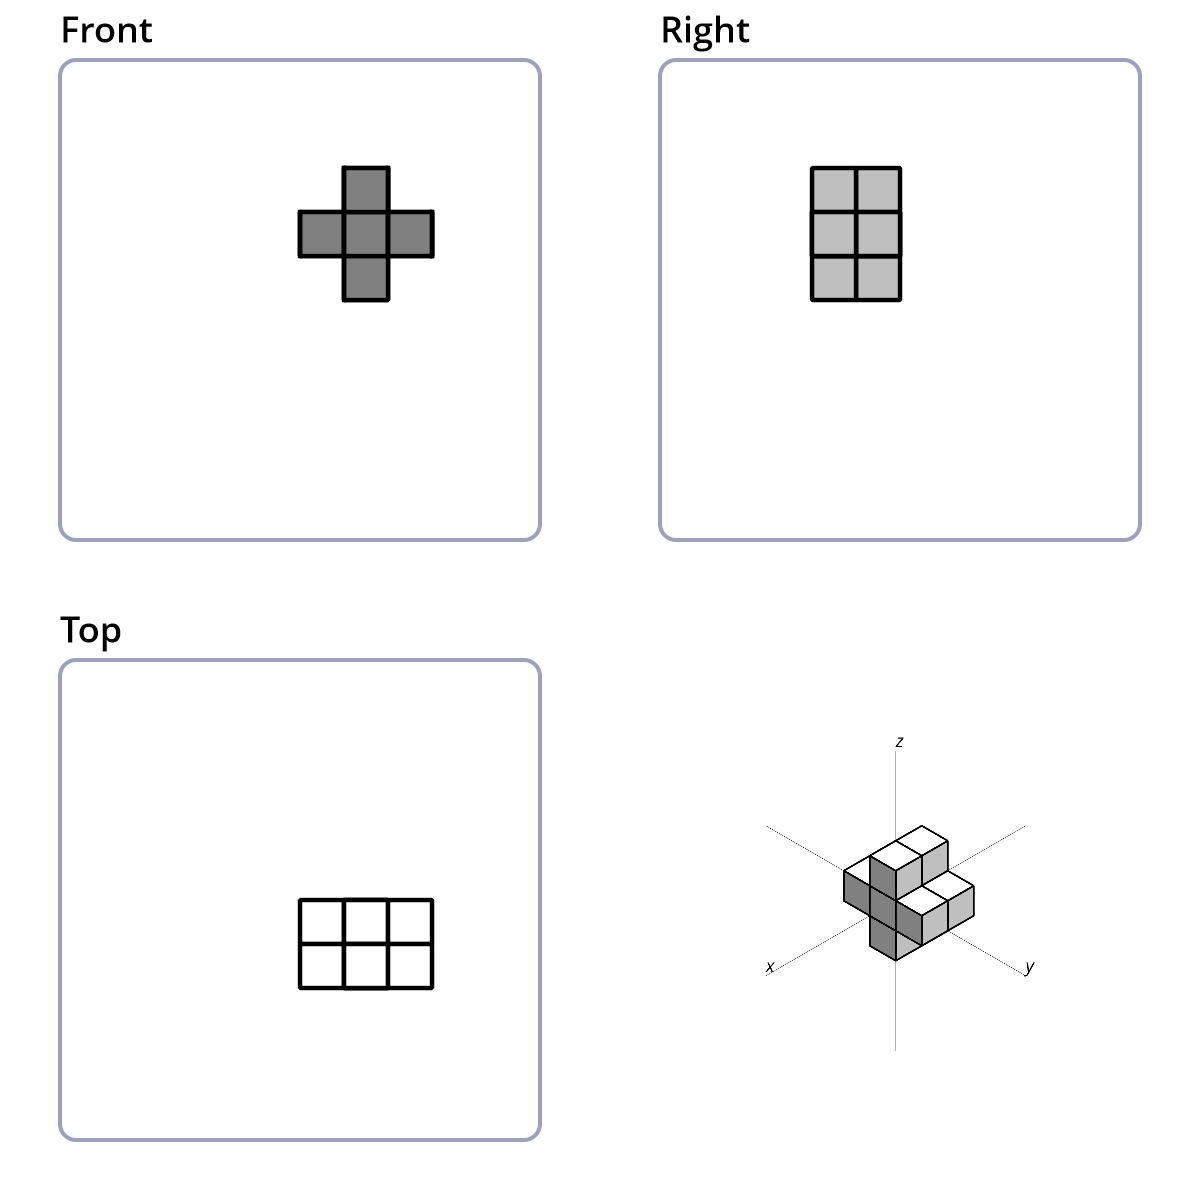
\includegraphics[scale=0.3]{iso_diagrams/x.png}
	\caption{Isometric of the X-pentomino.}
  \label{fig:iso-pent-x}
\end{figure}

\begin{figure}
	\centering
	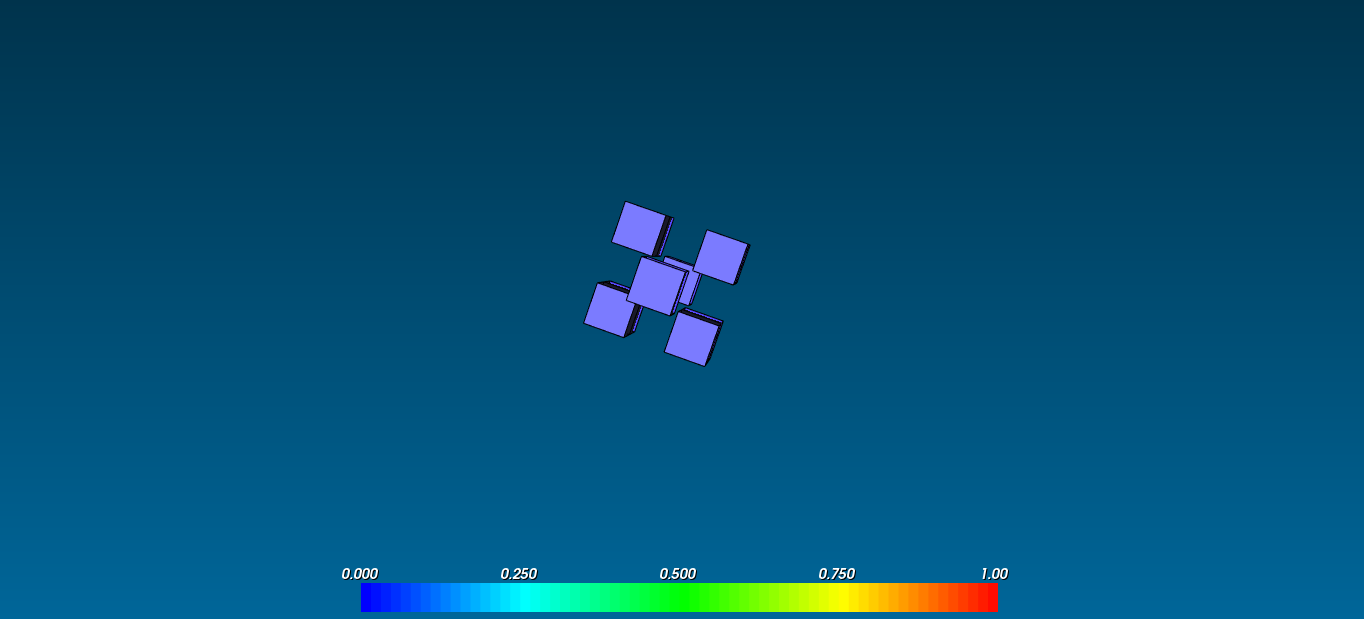
\includegraphics[scale=0.3]{pentominoes_ss/x_2.png}
	\caption{Evolution of the X-Pentomino, $2^{nd}$ generation.}
	\label{fig:ss-pent:x-2}
\end{figure}

\begin{figure}
	\centering
	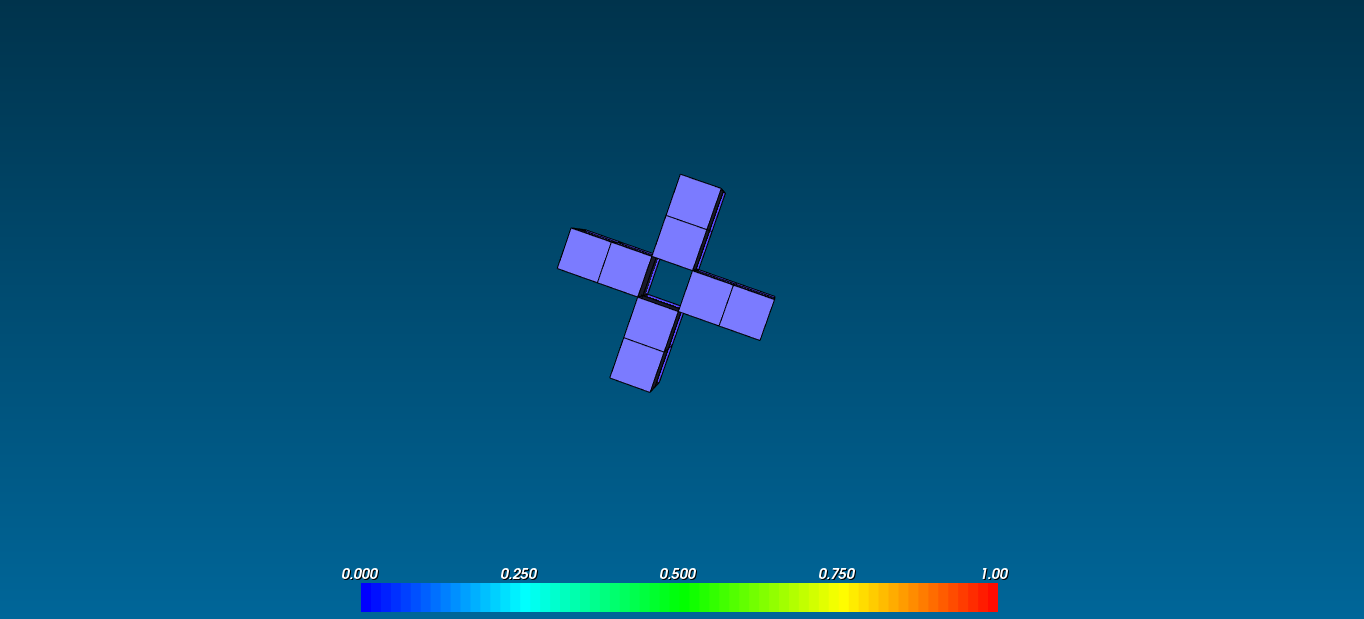
\includegraphics[scale=0.3]{pentominoes_ss/x_3.png}
	\caption{Evolution of the X-Pentomino, $3^{th}$ generation.}
	\label{fig:ss-pent:x-3}
\end{figure}

\begin{figure}
	\centering
	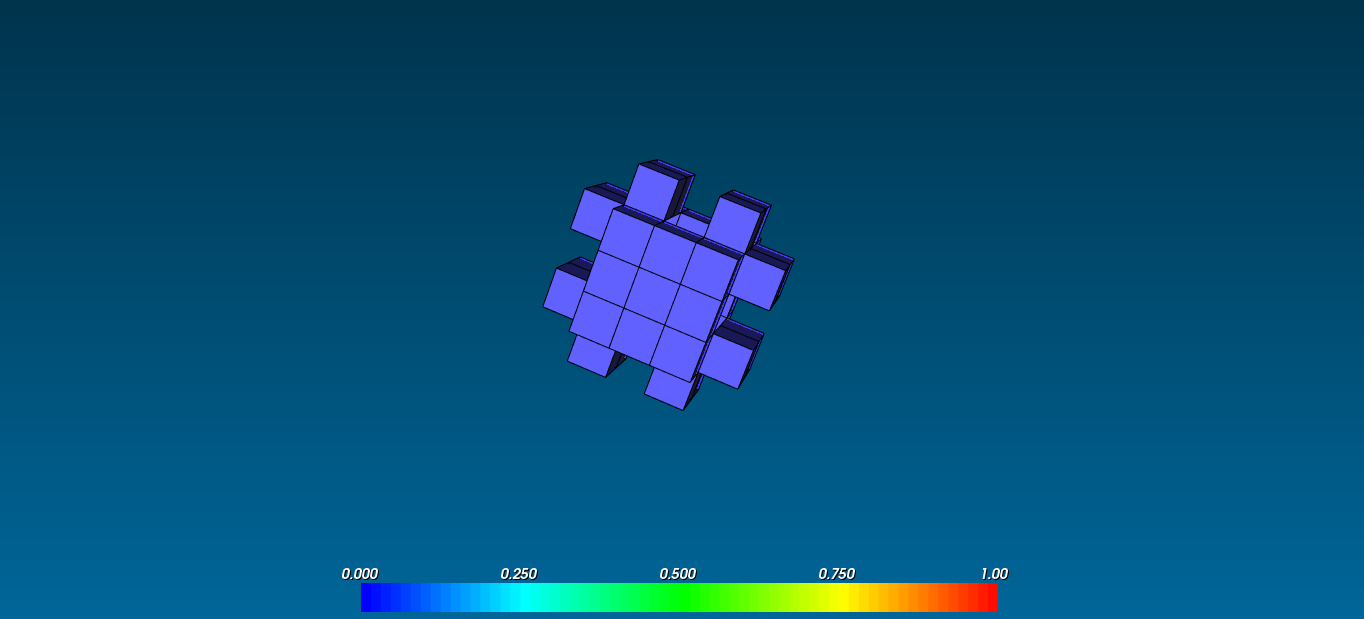
\includegraphics[scale=0.3]{pentominoes_ss/x_4.png}
	\caption{Evolution of the X-Pentomino, $4^{th}$ generation.}
	\label{fig:ss-pent:x-4}
\end{figure}

\begin{figure}
	\centering
	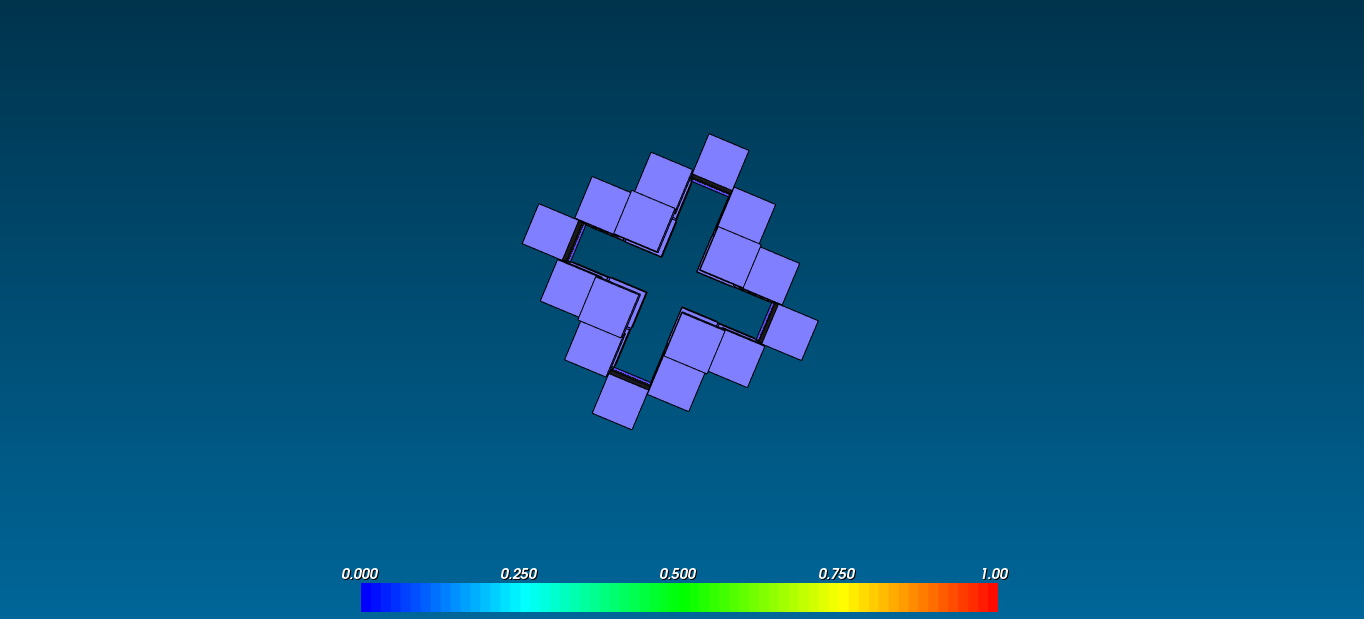
\includegraphics[scale=0.3]{pentominoes_ss/x_5.png}
	\caption{Evolution of the X-Pentomino, $5^{th}$ generation.}
	\label{fig:ss-pent:x-5}
\end{figure}

\begin{figure}
	\centering
	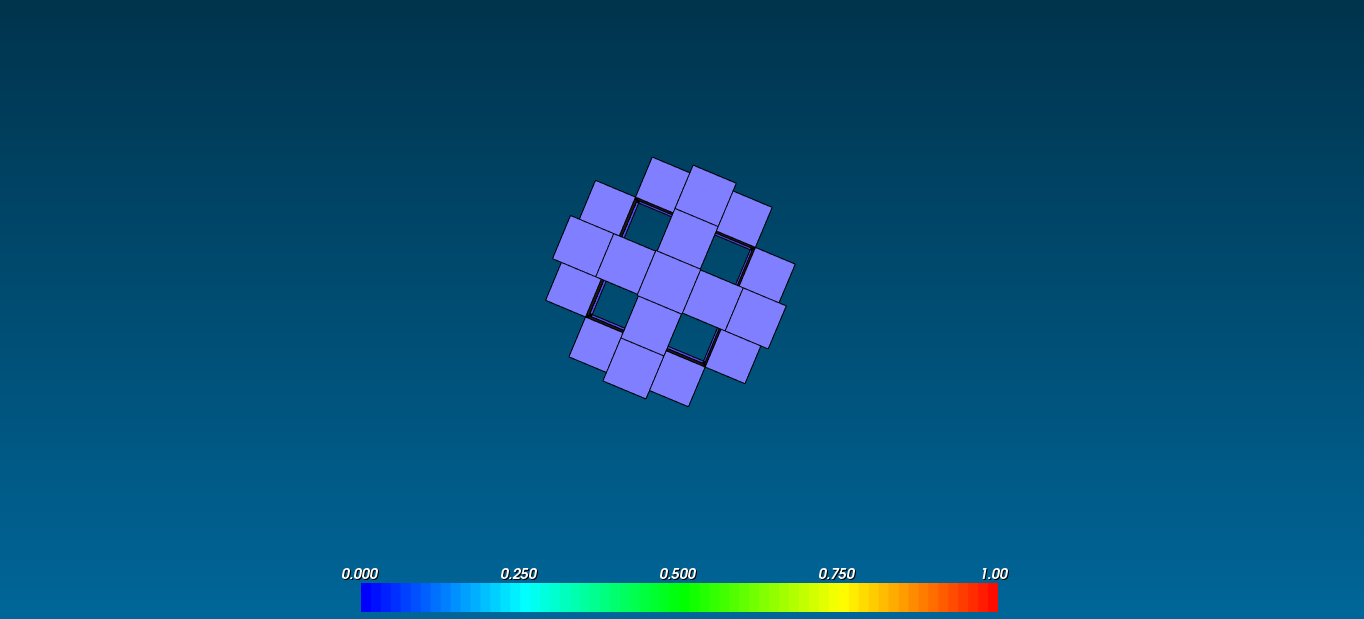
\includegraphics[scale=0.3]{pentominoes_ss/x_6.png}
	\caption{Evolution of the X-Pentomino, $6^{th}$ generation.}
	\label{fig:ss-pent:x-6}
\end{figure}

\begin{figure}
	\centering
	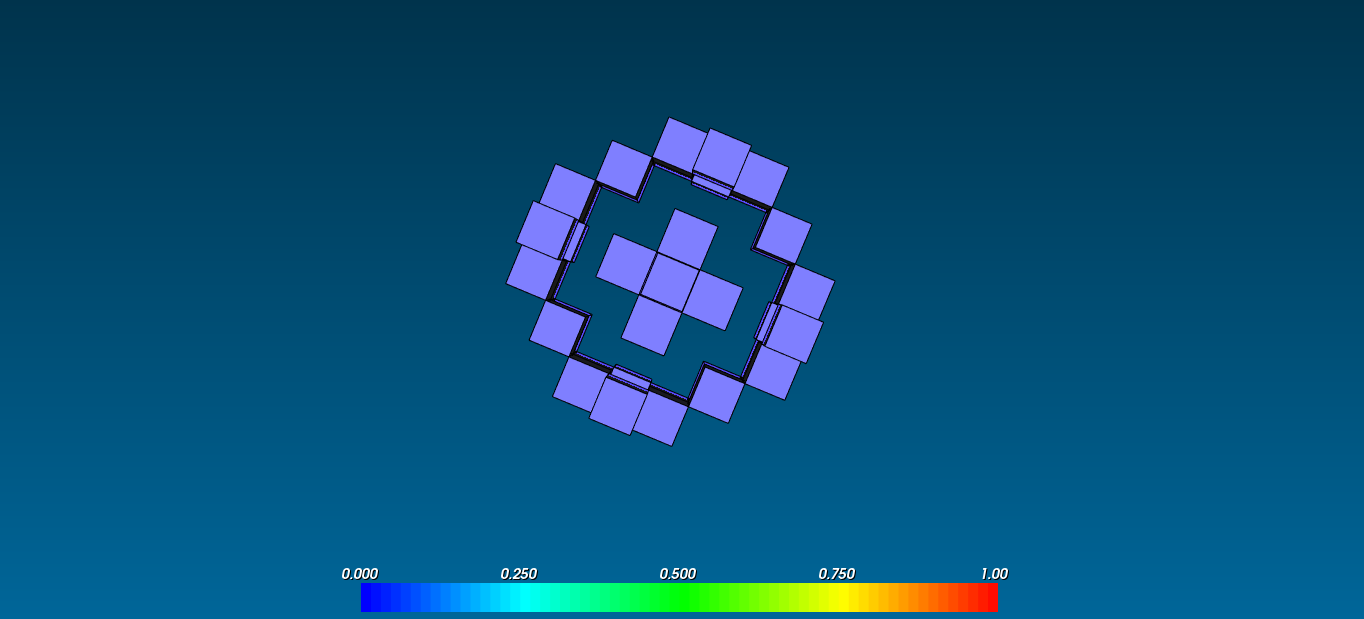
\includegraphics[scale=0.3]{pentominoes_ss/x_7.png}
	\caption{Evolution of the X-Pentomino, $7^{th}$ generation.}
	\label{fig:ss-pent:x-7}
\end{figure}

\begin{figure}
	\centering
	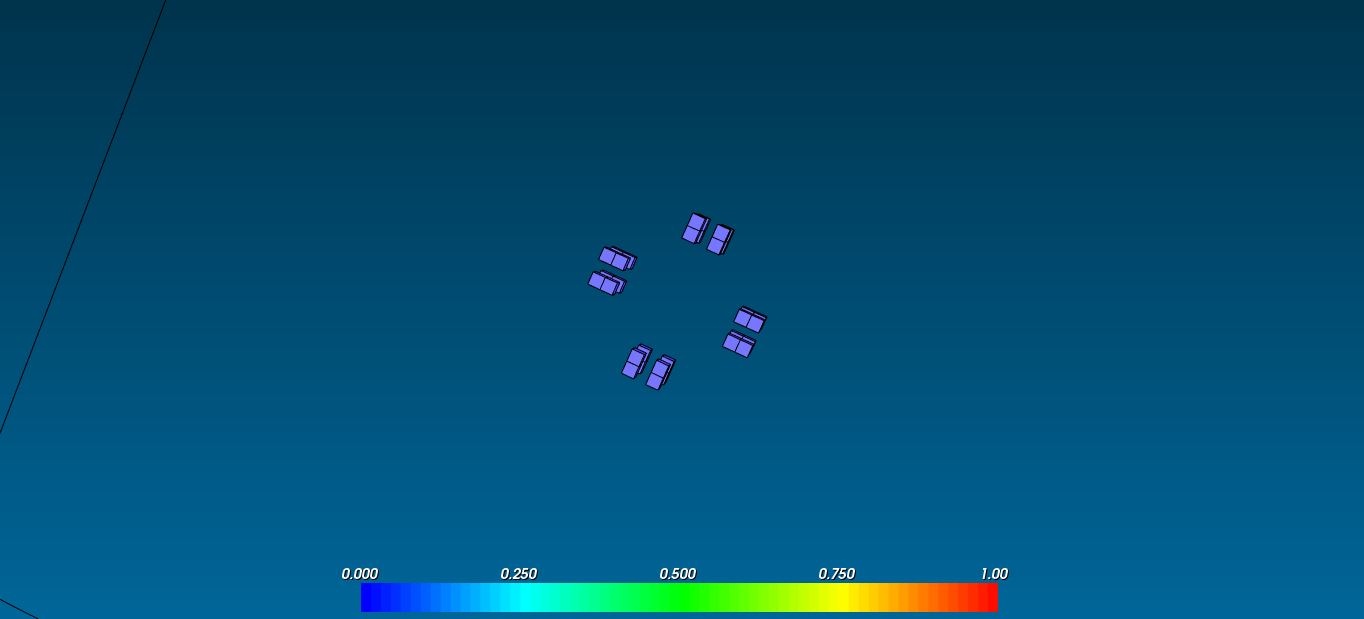
\includegraphics[scale=0.3]{pentominoes_ss/x_15.png}
	\caption{Evolution of the X-Pentomino, $15^{th}$ generation.}
	\label{fig:ss-pent:x-15}
\end{figure}

% Y PENTOMINO ==================================================================
\subsubsection{Y-Pentomino}
\label{sec:y-pentomino}
This pentomino (see figure~\ref{fig:iso-pent-y}),


\begin{figure}
	\centering
	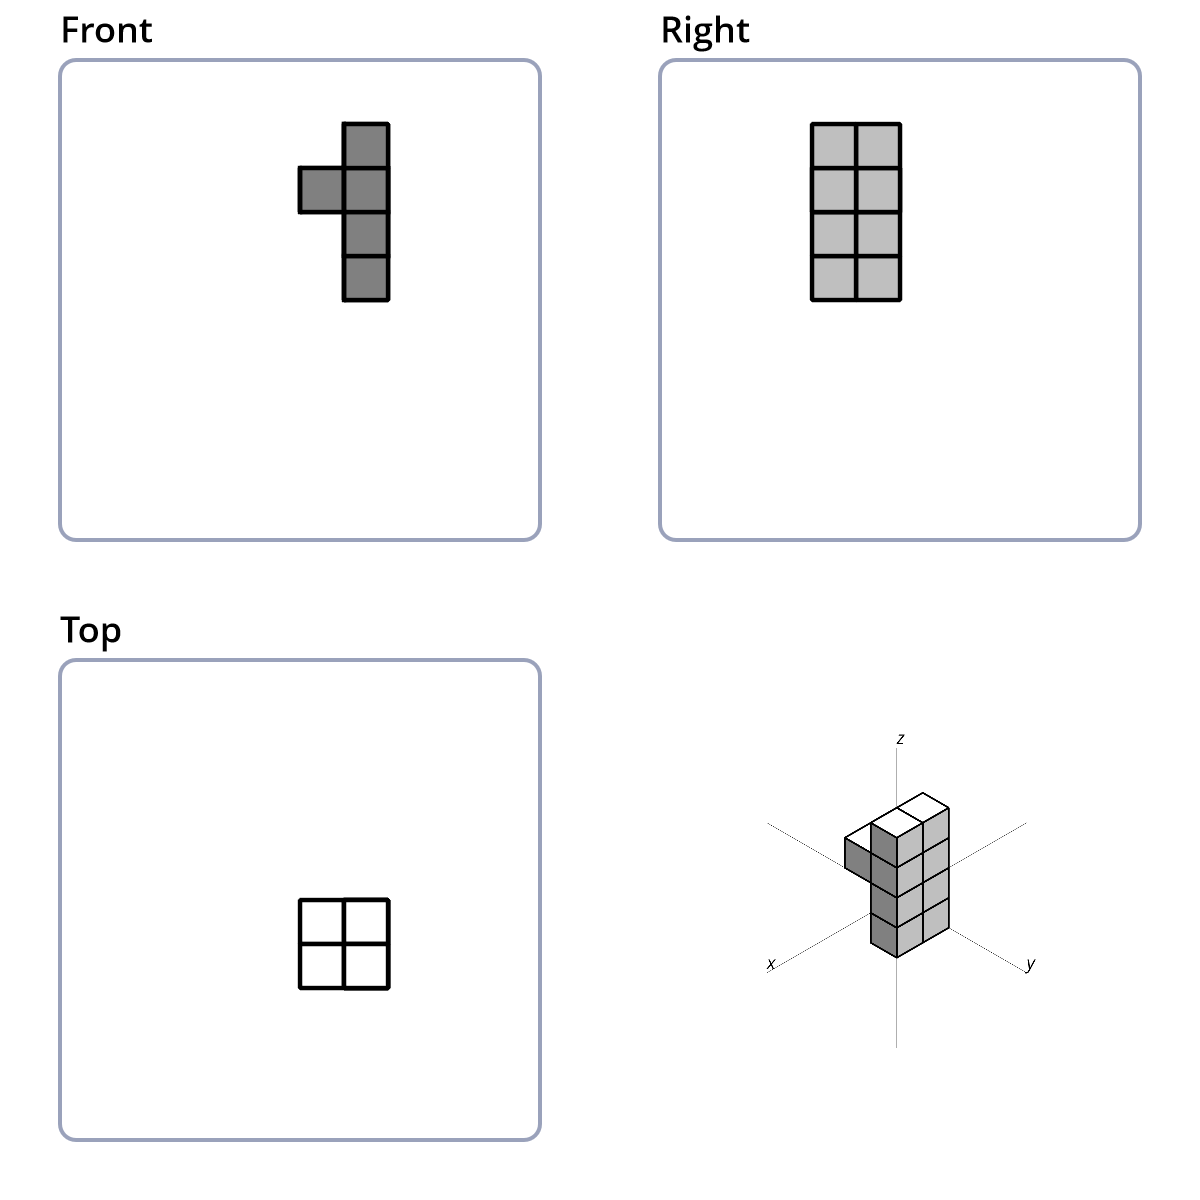
\includegraphics[scale=0.3]{iso_diagrams/y.png}
	\caption{Isometric of the Y-pentomino.}
  \label{fig:iso-pent-y}
\end{figure}

% Z PENTOMINO ==================================================================
\subsubsection{Z-Pentomino}
\label{sec:z-pentomino}
This pentomino (see figure~\ref{fig:iso-pent-z}),


\begin{figure}
	\centering
	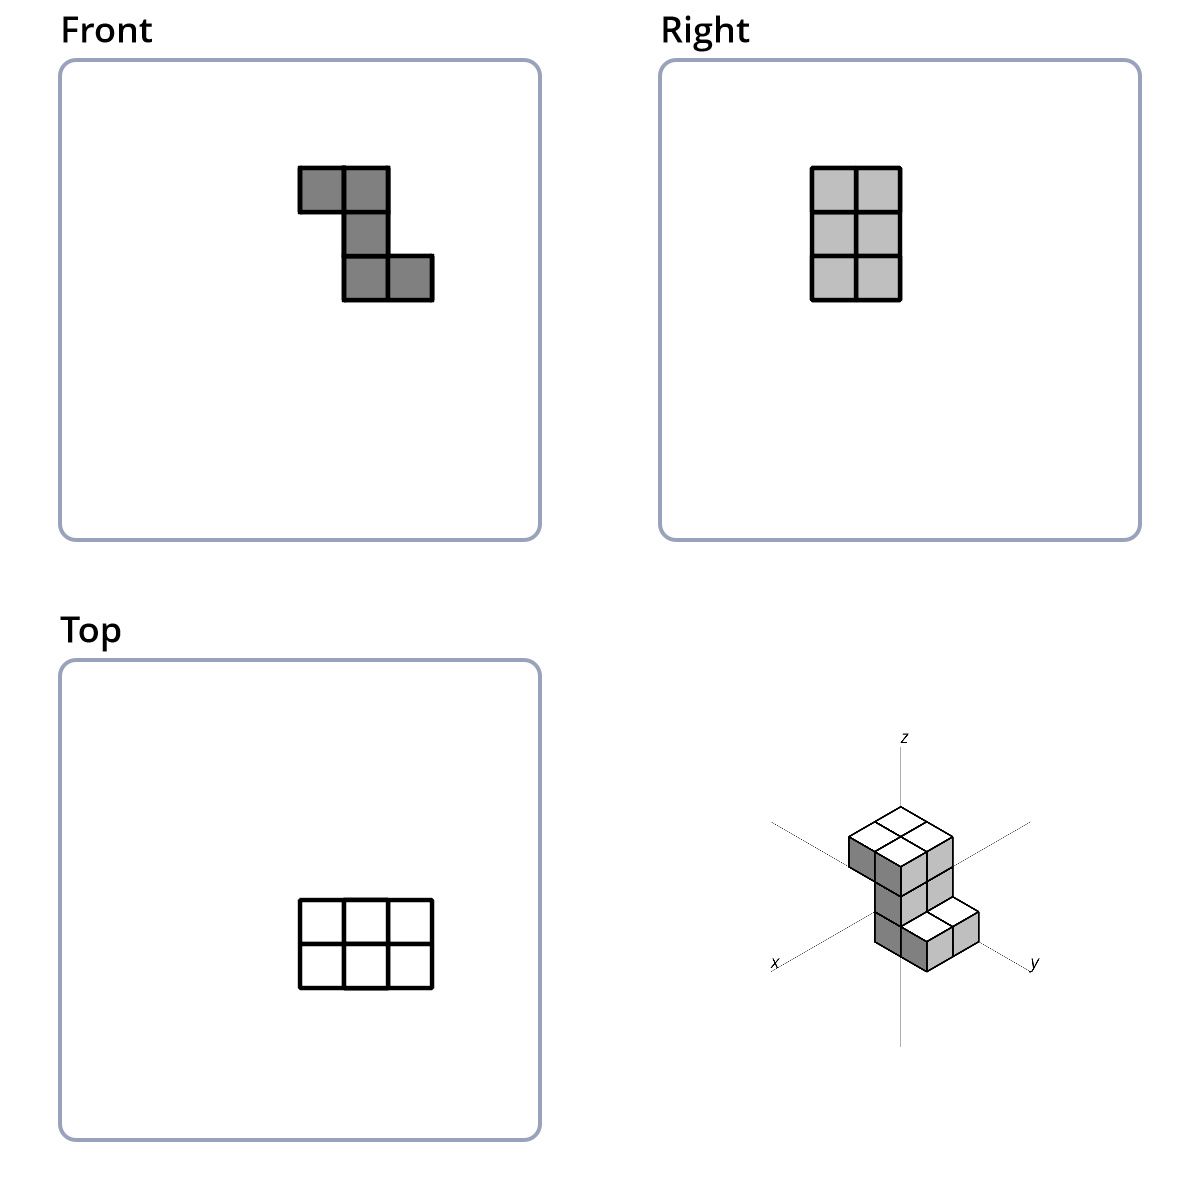
\includegraphics[scale=0.3]{iso_diagrams/z.png}
	\caption{Isometric of the Z-pentomino.}
  \label{fig:iso-pent-z}
\end{figure}
